\section{Numerical examples}

\subsection{Inf--sup test}

\begin{figure}[!ht]
\centering

\includegraphics[width=0.5\textwidth]{png/infsup_model.png}
\caption{Illustration of inf--sup test}\label{infsup_illsutration}
\end{figure}

\subsubsection{Inf--sup test}

\begin{figure}[!ht]
\centering
\begin{subcaptiongroup}
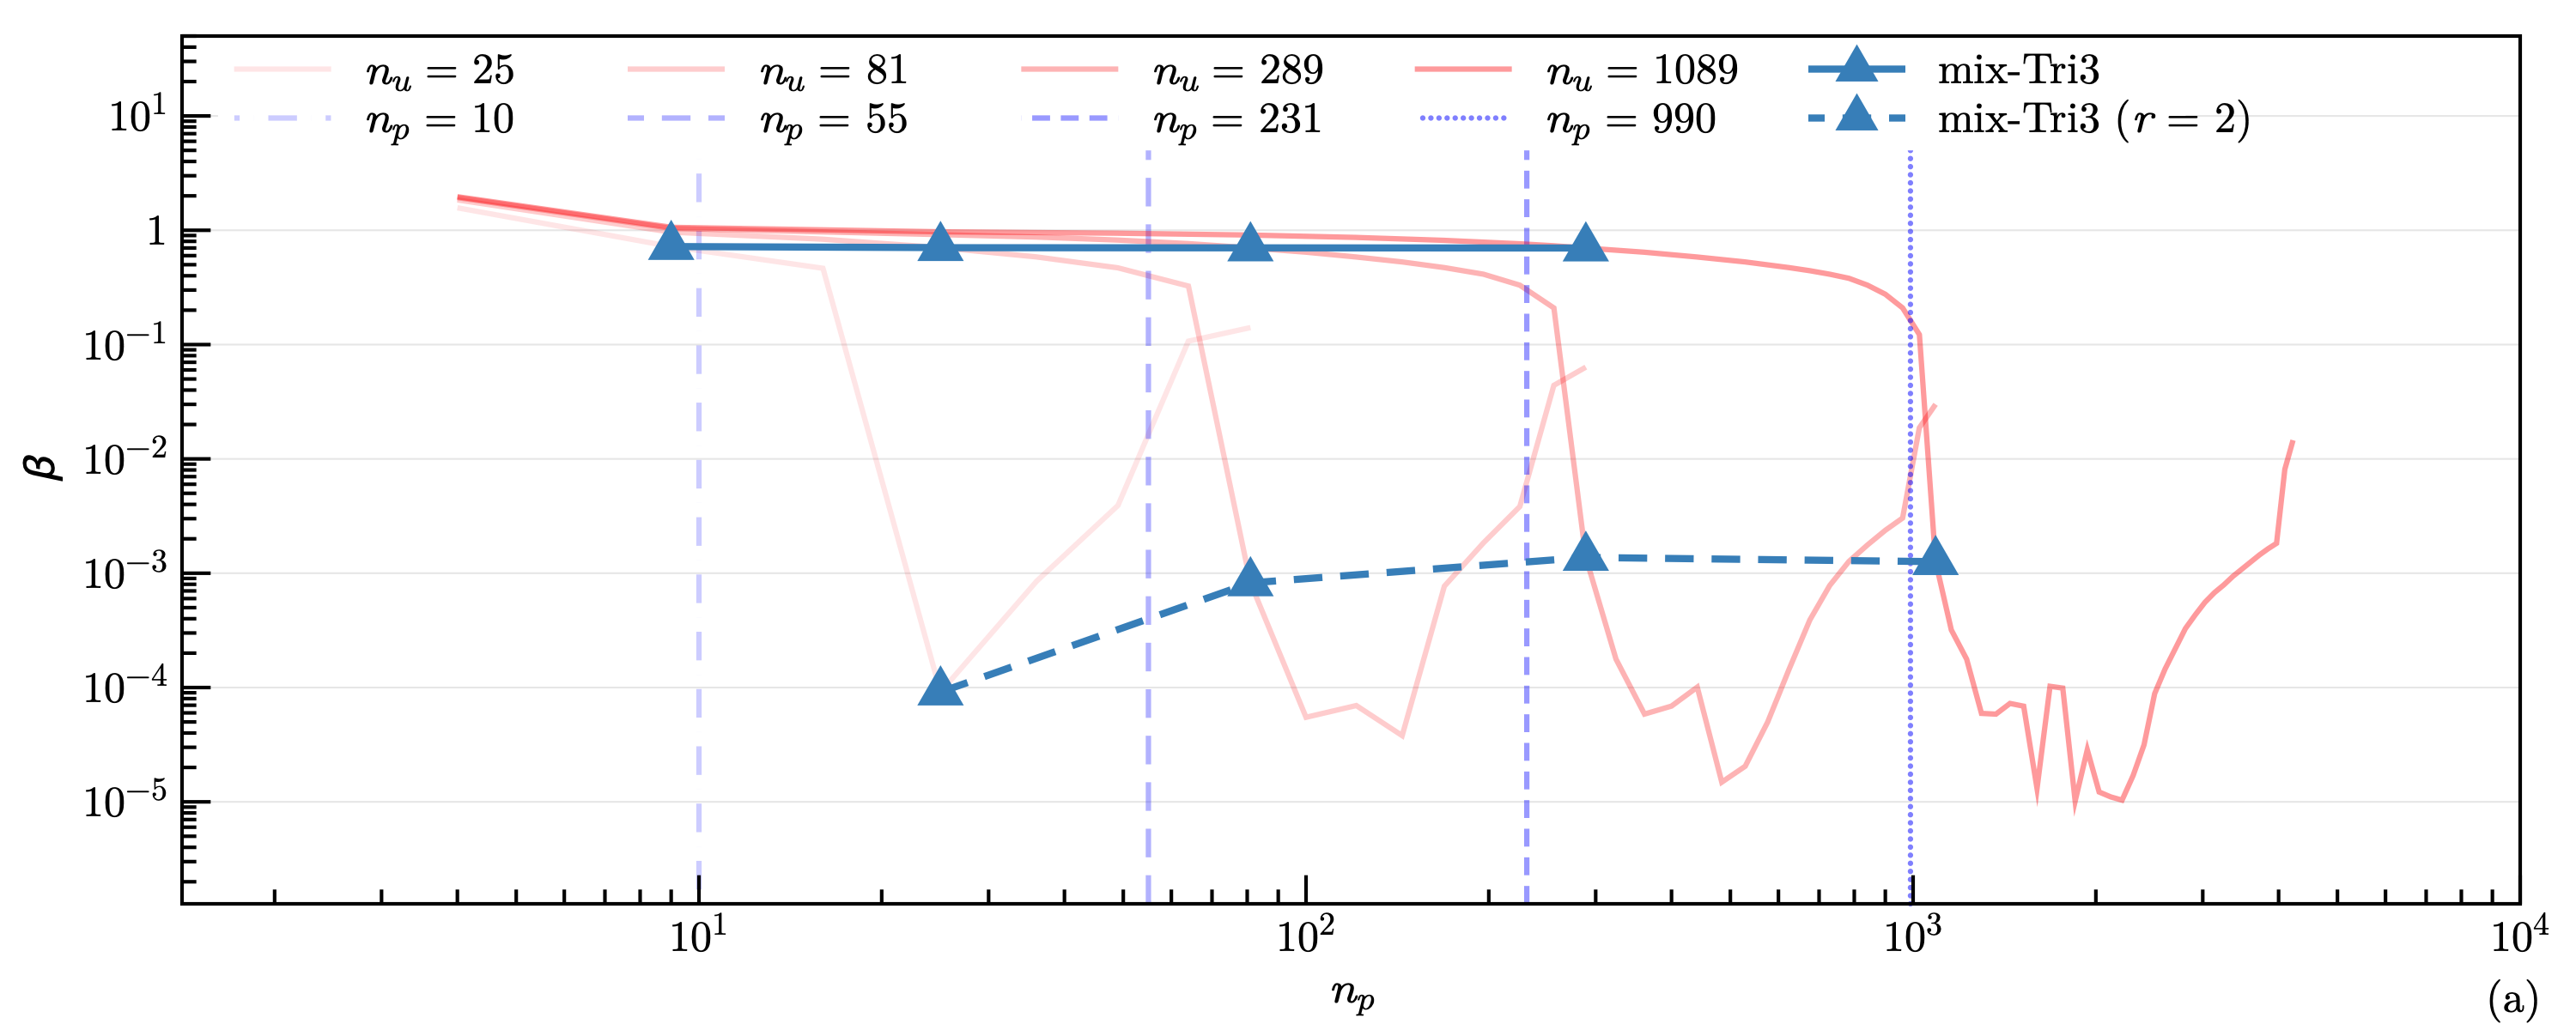
\includegraphics[width=\textwidth]{png/infsup_tri3.png}\phantomcaption\label{a}
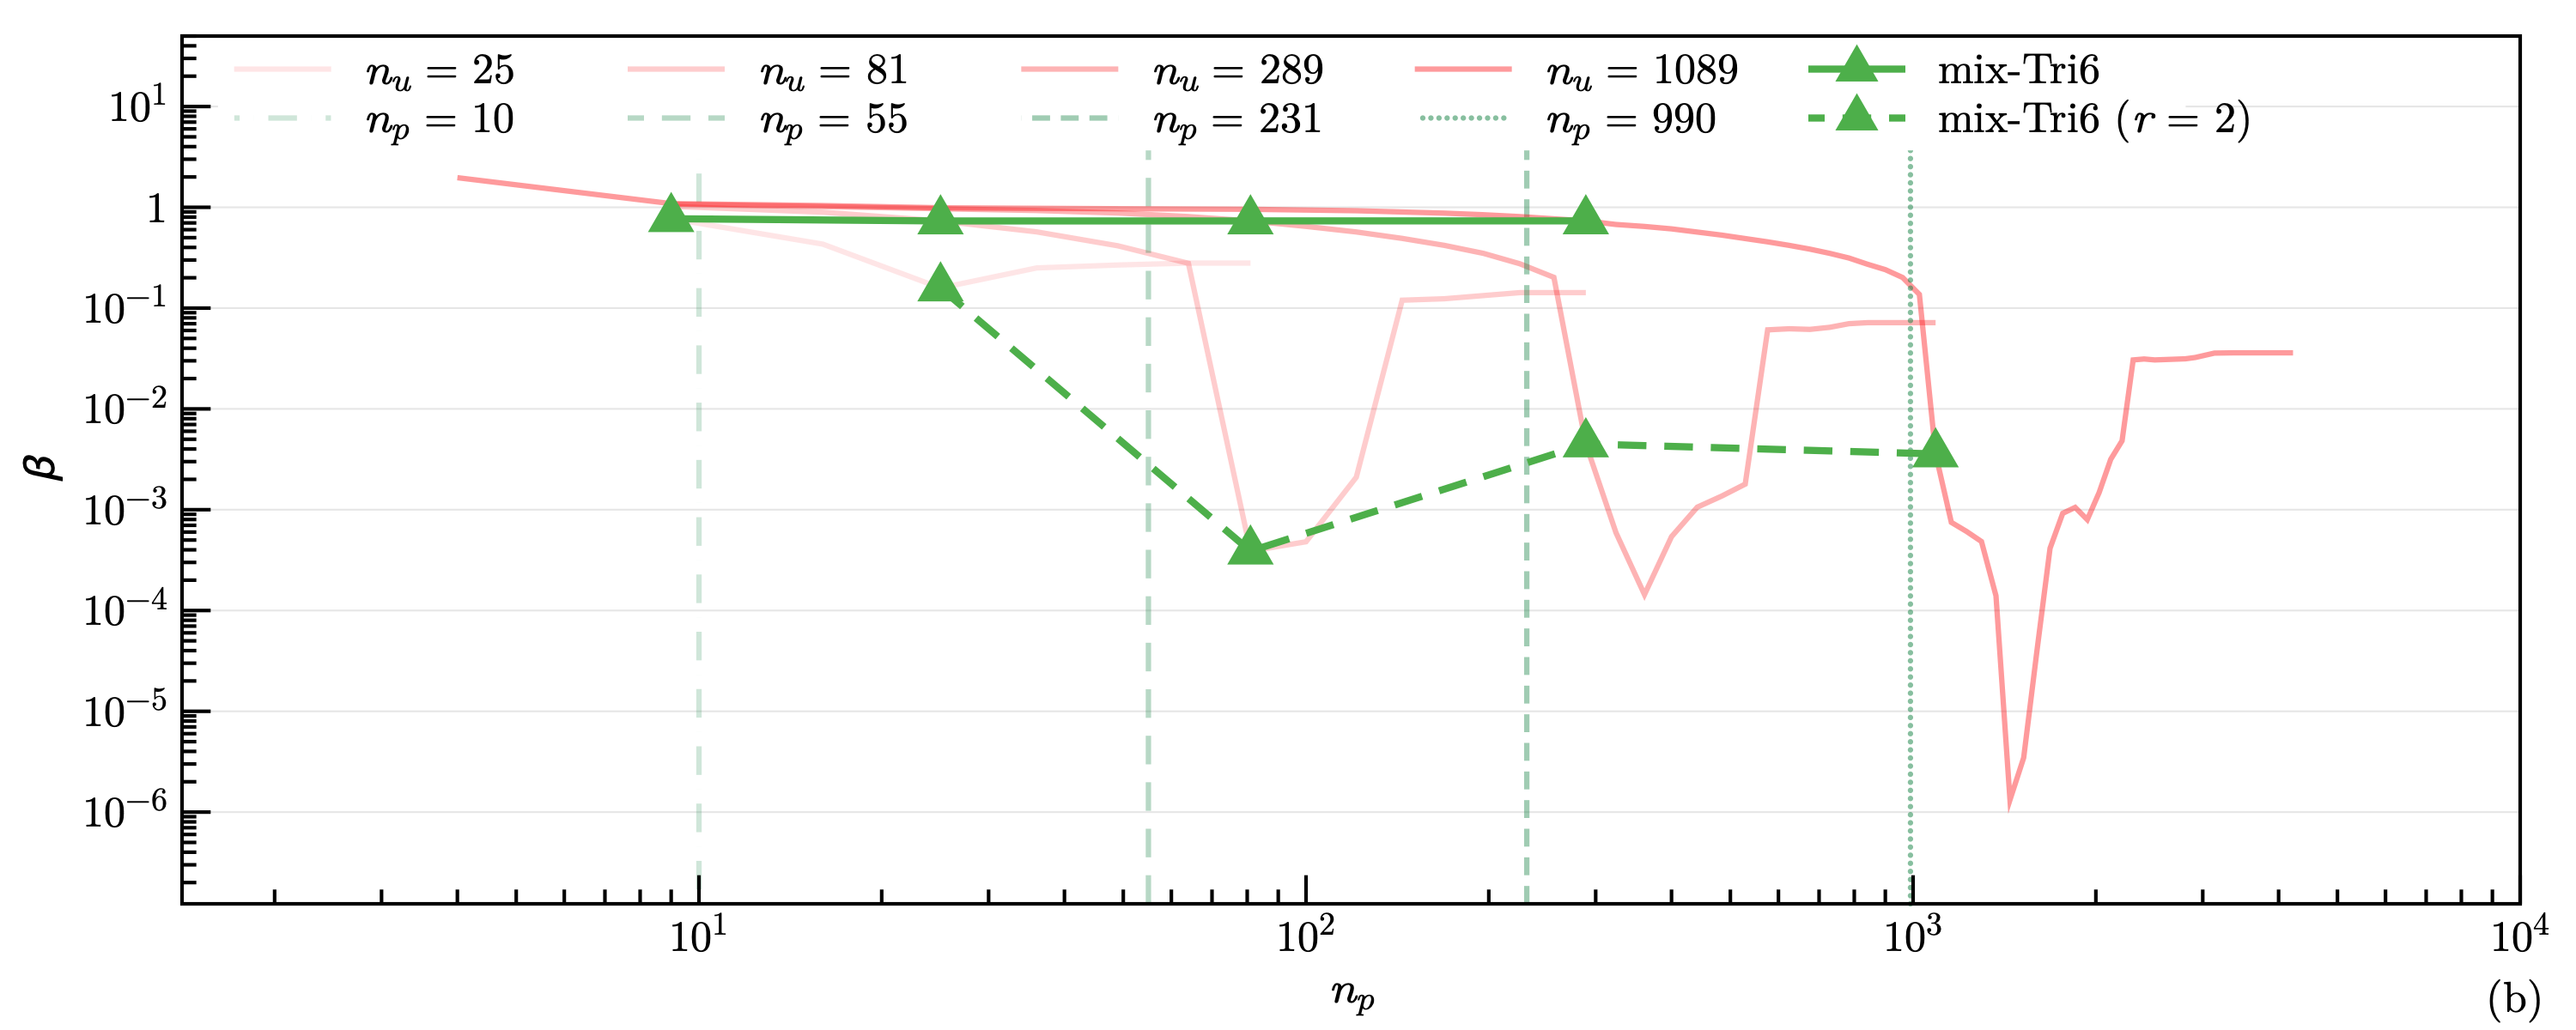
\includegraphics[width=\textwidth]{png/infsup_tri6.png}\phantomcaption\label{b}
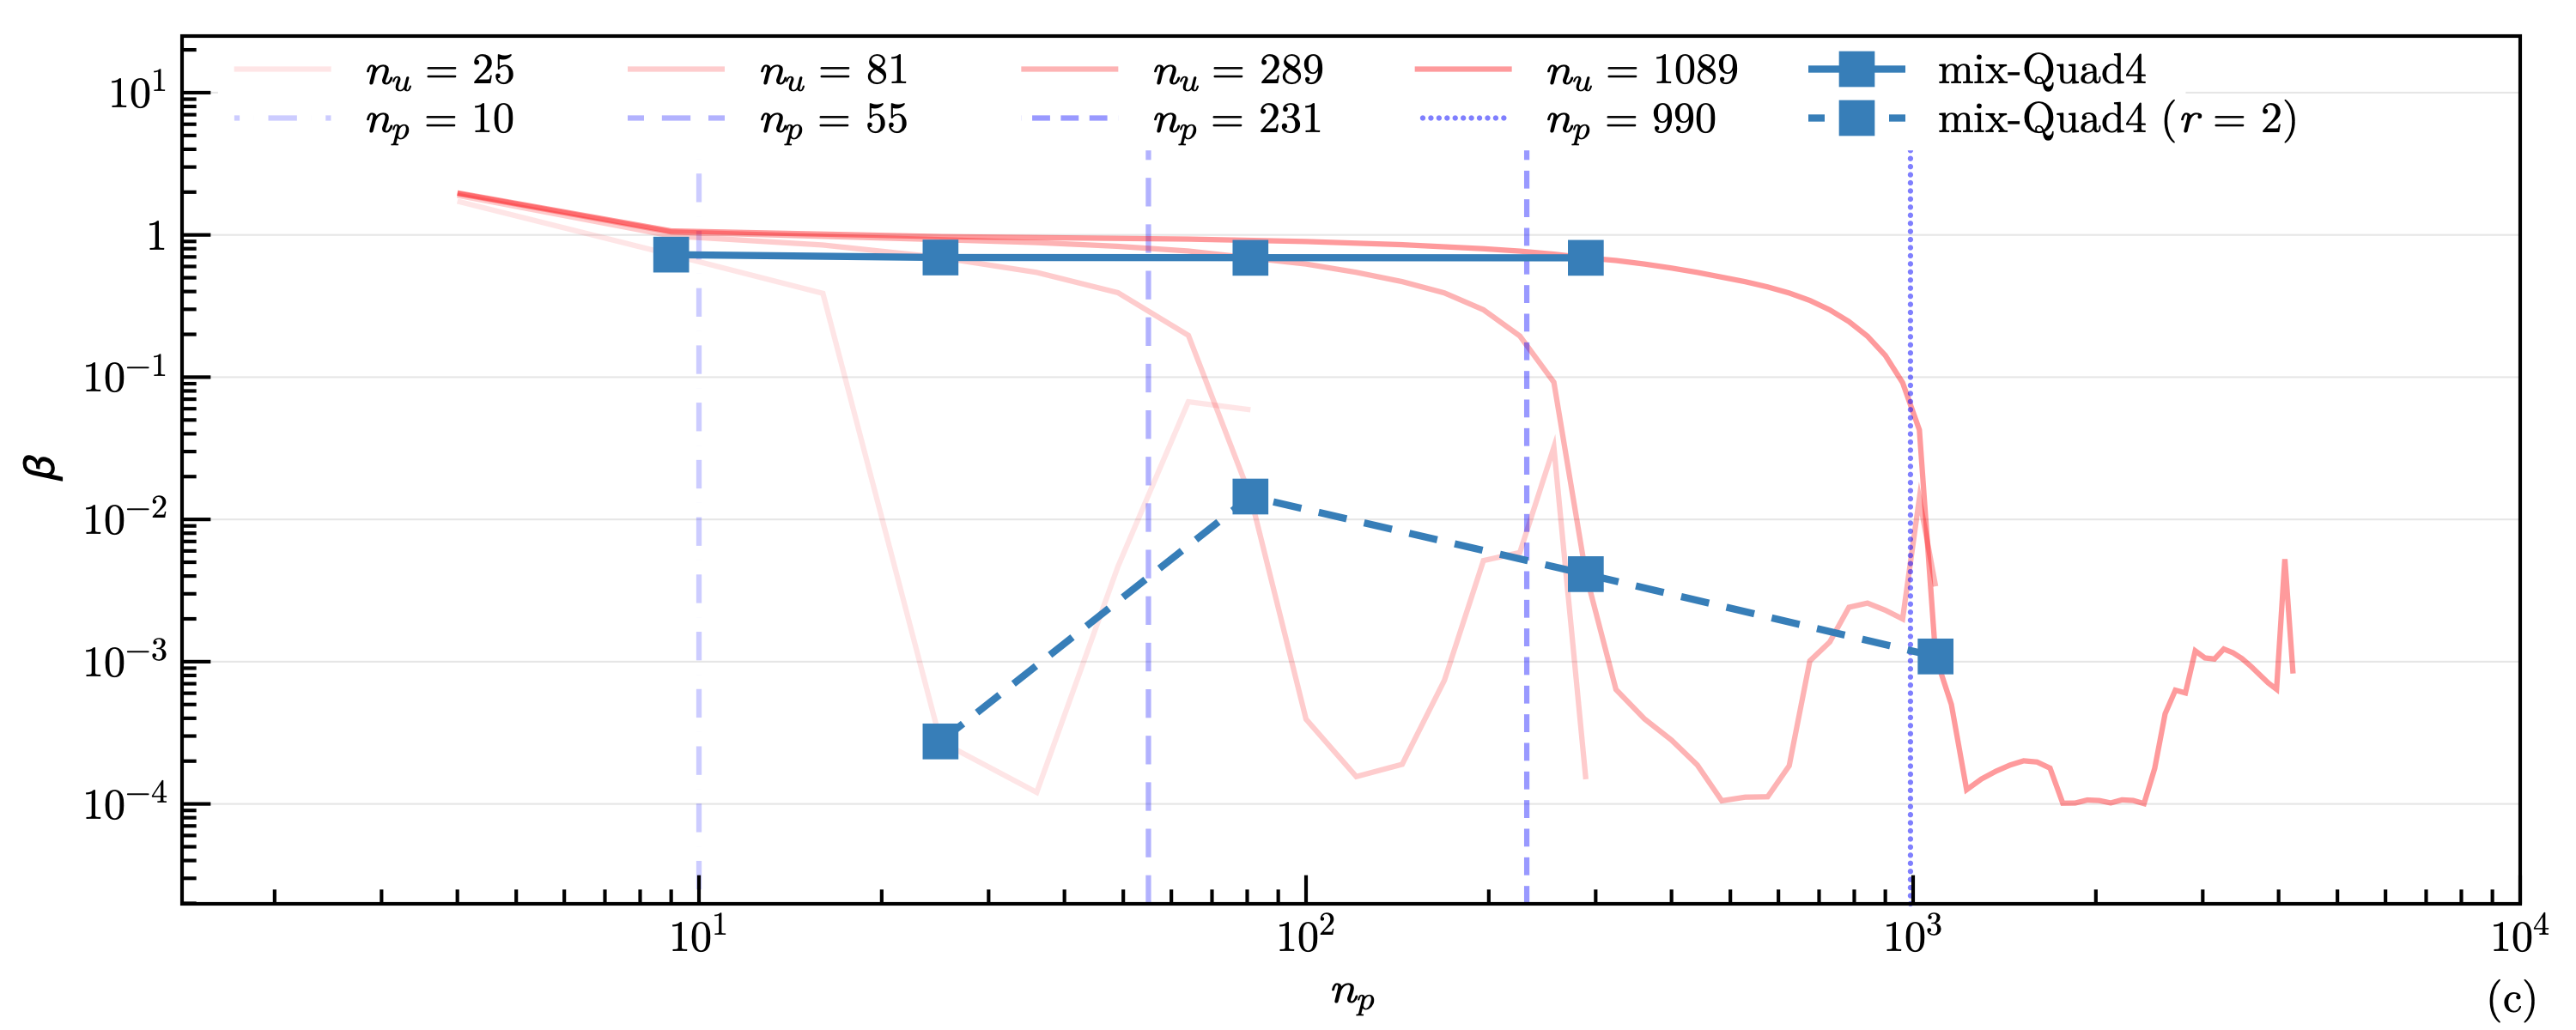
\includegraphics[width=\textwidth]{png/infsup_quad.png}\phantomcaption\label{c}
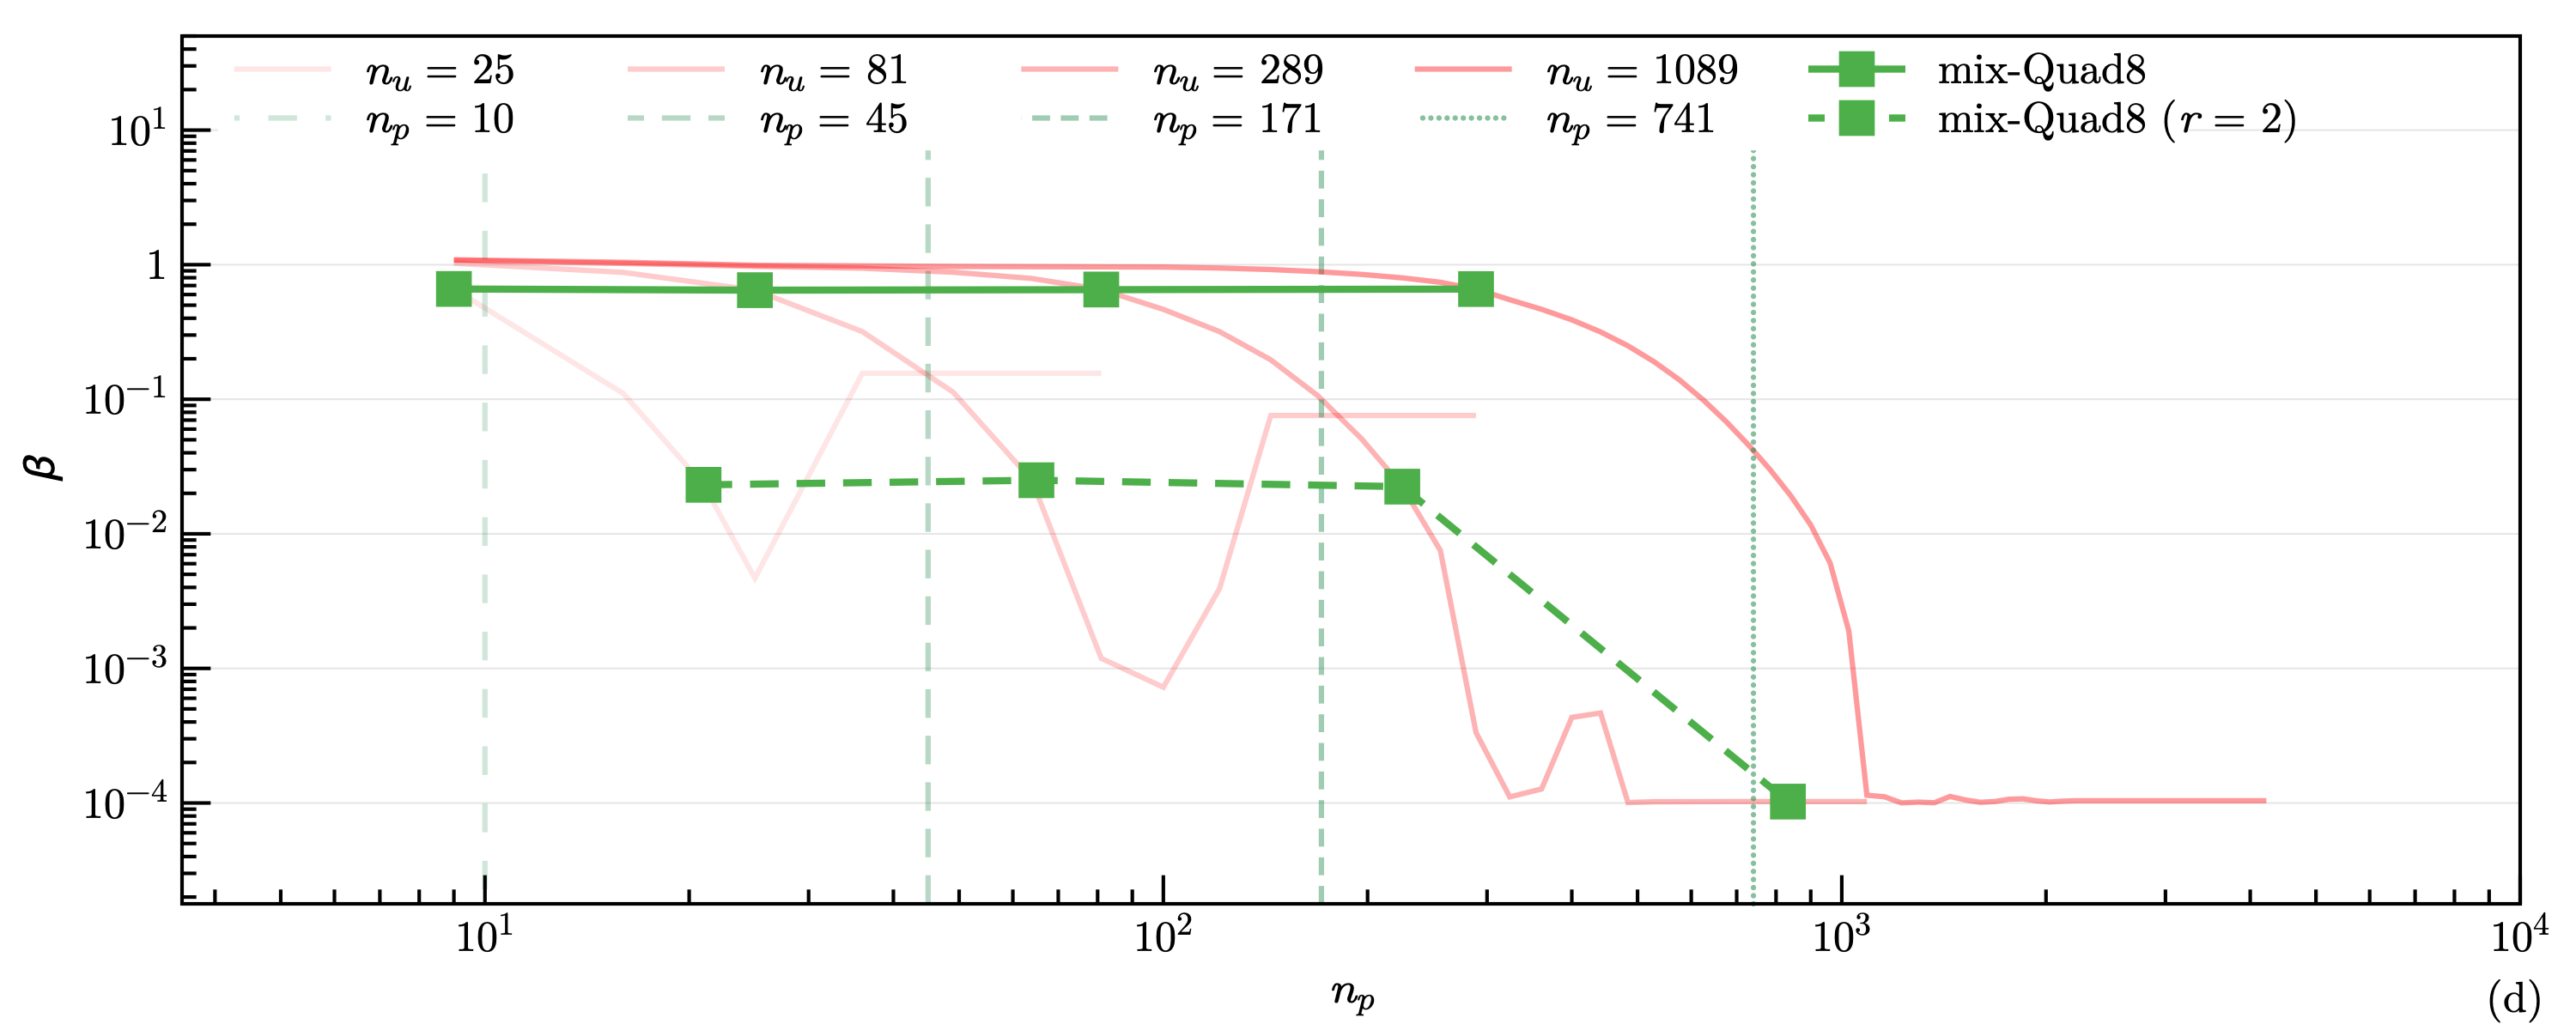
\includegraphics[width=\textwidth]{png/infsup_quad8.png}\phantomcaption\label{d}
\end{subcaptiongroup}
\captionsetup{aboveskip=0pt}
\caption{\centering Inf--sup test for various finite element formulations: \\ (\subref{a}) mix-Tri3; (\subref{b}) mix-Tri6; (\subref{c}) mix-Quad4; (\subref{d}) mix-Quad8}
\label{infsup_convergence}
\end{figure}

\begin{table}[!ht]
\centering
\caption{Results of Nearly--incompressible elasticity patch test}\label{patchtest_result}
\begin{tabular}{lcccc}
\toprule
 & \multicolumn{2}{c}{Linear patch test} & \multicolumn{2}{c}{Quadratic patch test} \\ \cline{2-5}
 & $L_2$-Error & $H_e$-Error & $L_2$-Error & $H_e$-Error \\
\midrule
    T3-stripe & & & & \\
    T3-cross & & & & \\
    T3-mix & & & & \\
    Q4 & & & & \\
    Q4R1 & & & & \\
    Q4-mix & & & \\
    T6 & & & & \\
    T6P3 & & & & \\
    T6-mix & & & & \\
    Q8 & & & & \\
    Q8P3 & & & & \\
    Q8-mix & & & & \\
\bottomrule
\end{tabular}
\end{table}

\subsection{Cantilever beam problem}

\begin{figure}[!ht]
\centering
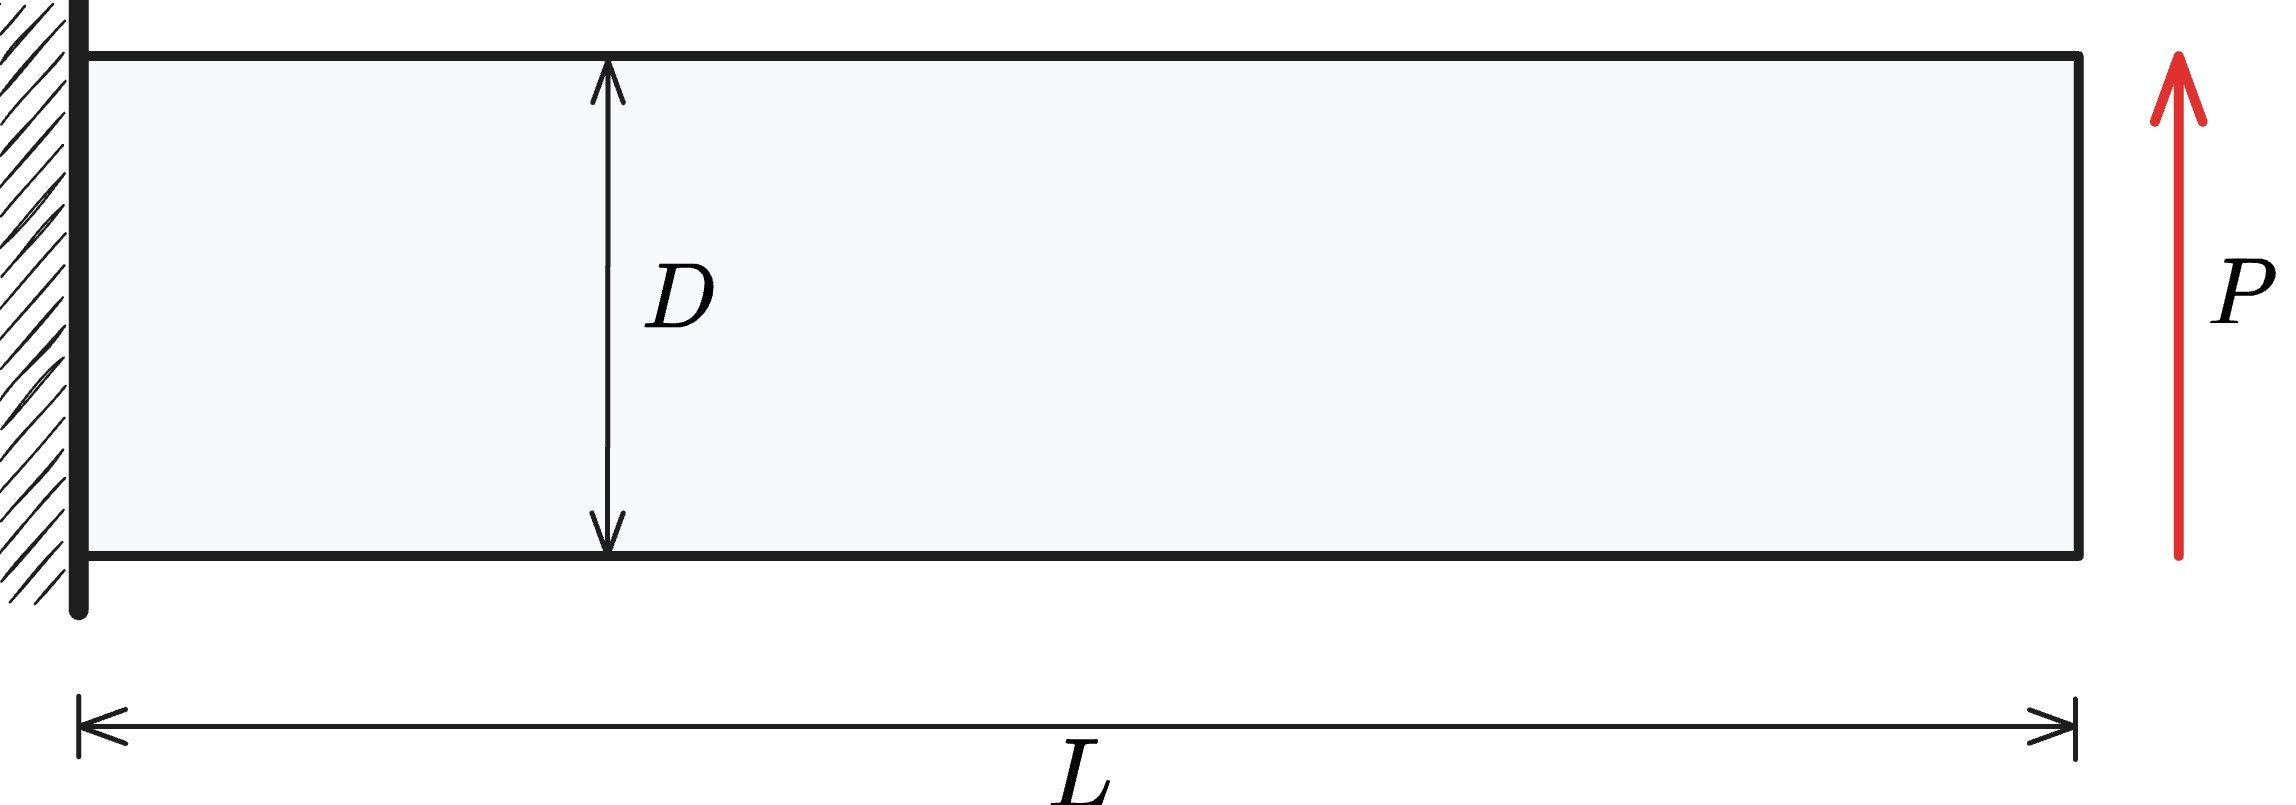
\includegraphics[width=0.8\textwidth]{png/cantilever_model.png}
\caption{Illustration of cantilever beam problem}\label{cantilever_1}
\end{figure}

\begin{figure}[!ht]
\centering
\begin{subcaptiongroup}
    \begin{tabular}{c@{\hspace{0pt}}c@{\hspace{0pt}}c}
      $\Vert \boldsymbol u - \boldsymbol u_h \Vert_V$ & $\Vert p - p_h \Vert_Q$ & \\
      \raisebox{-0.8\height}{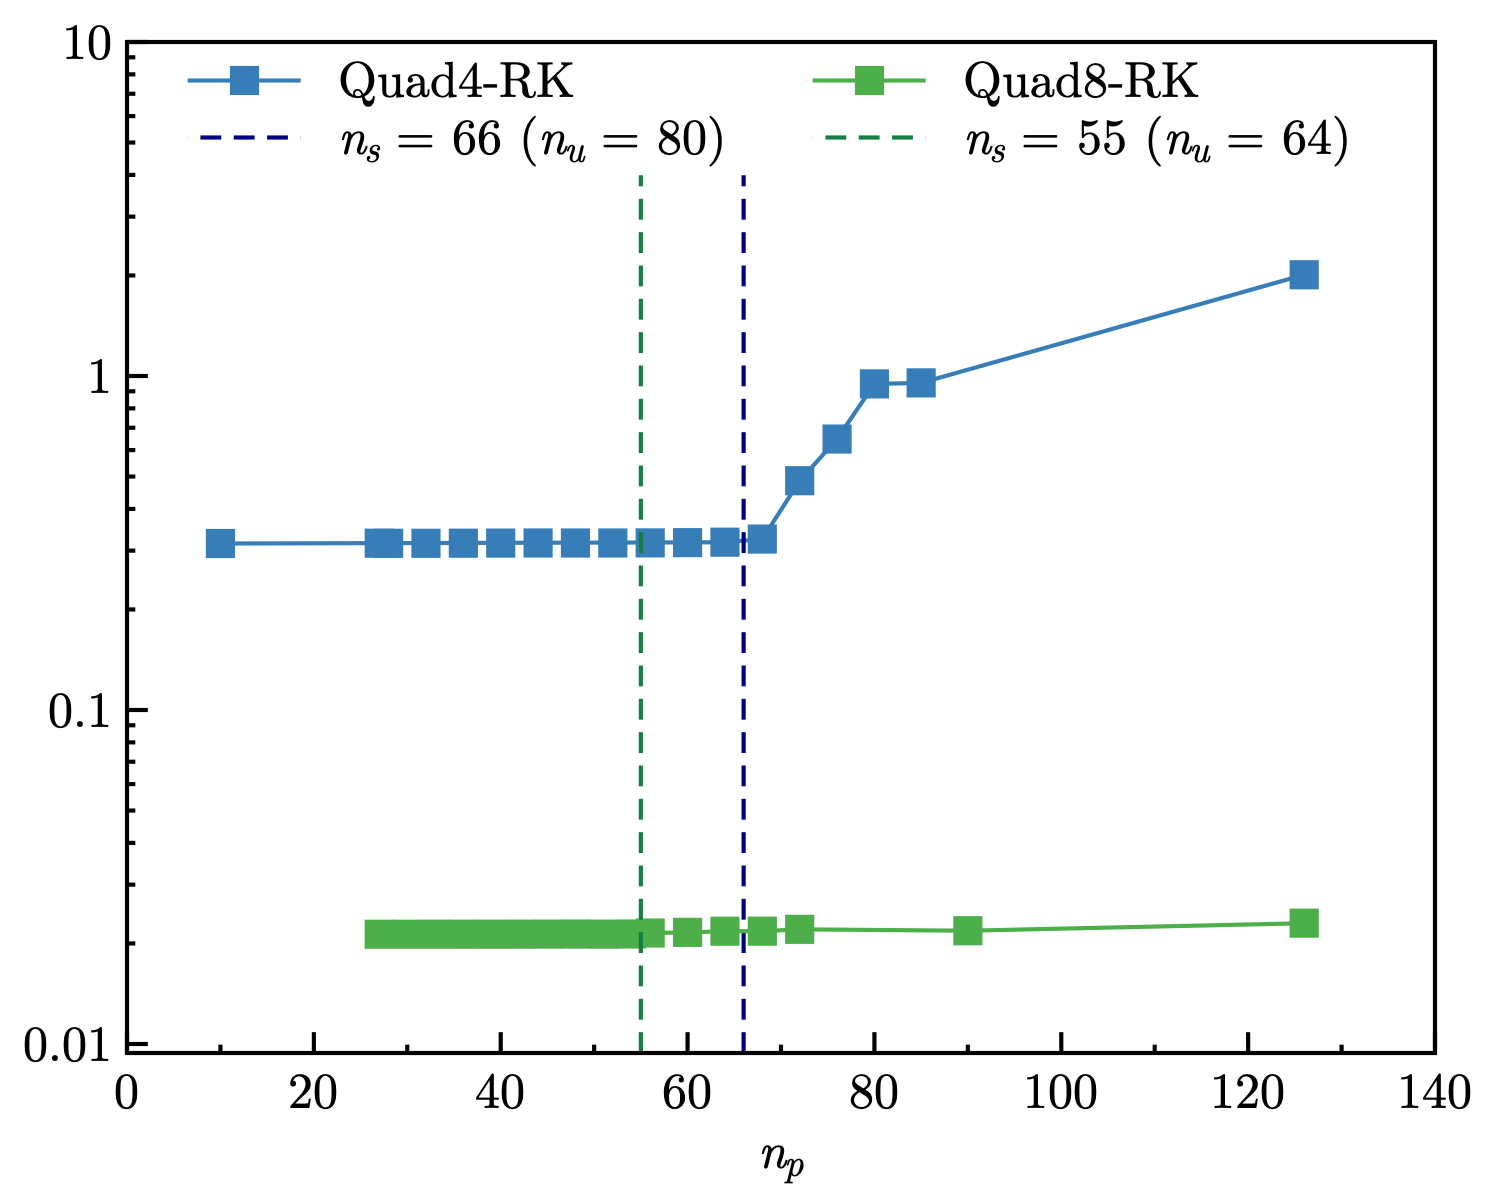
\includegraphics[width=0.45\textwidth]{png/cantilever_Hdev_4.png}}
    & \raisebox{-0.8\height}{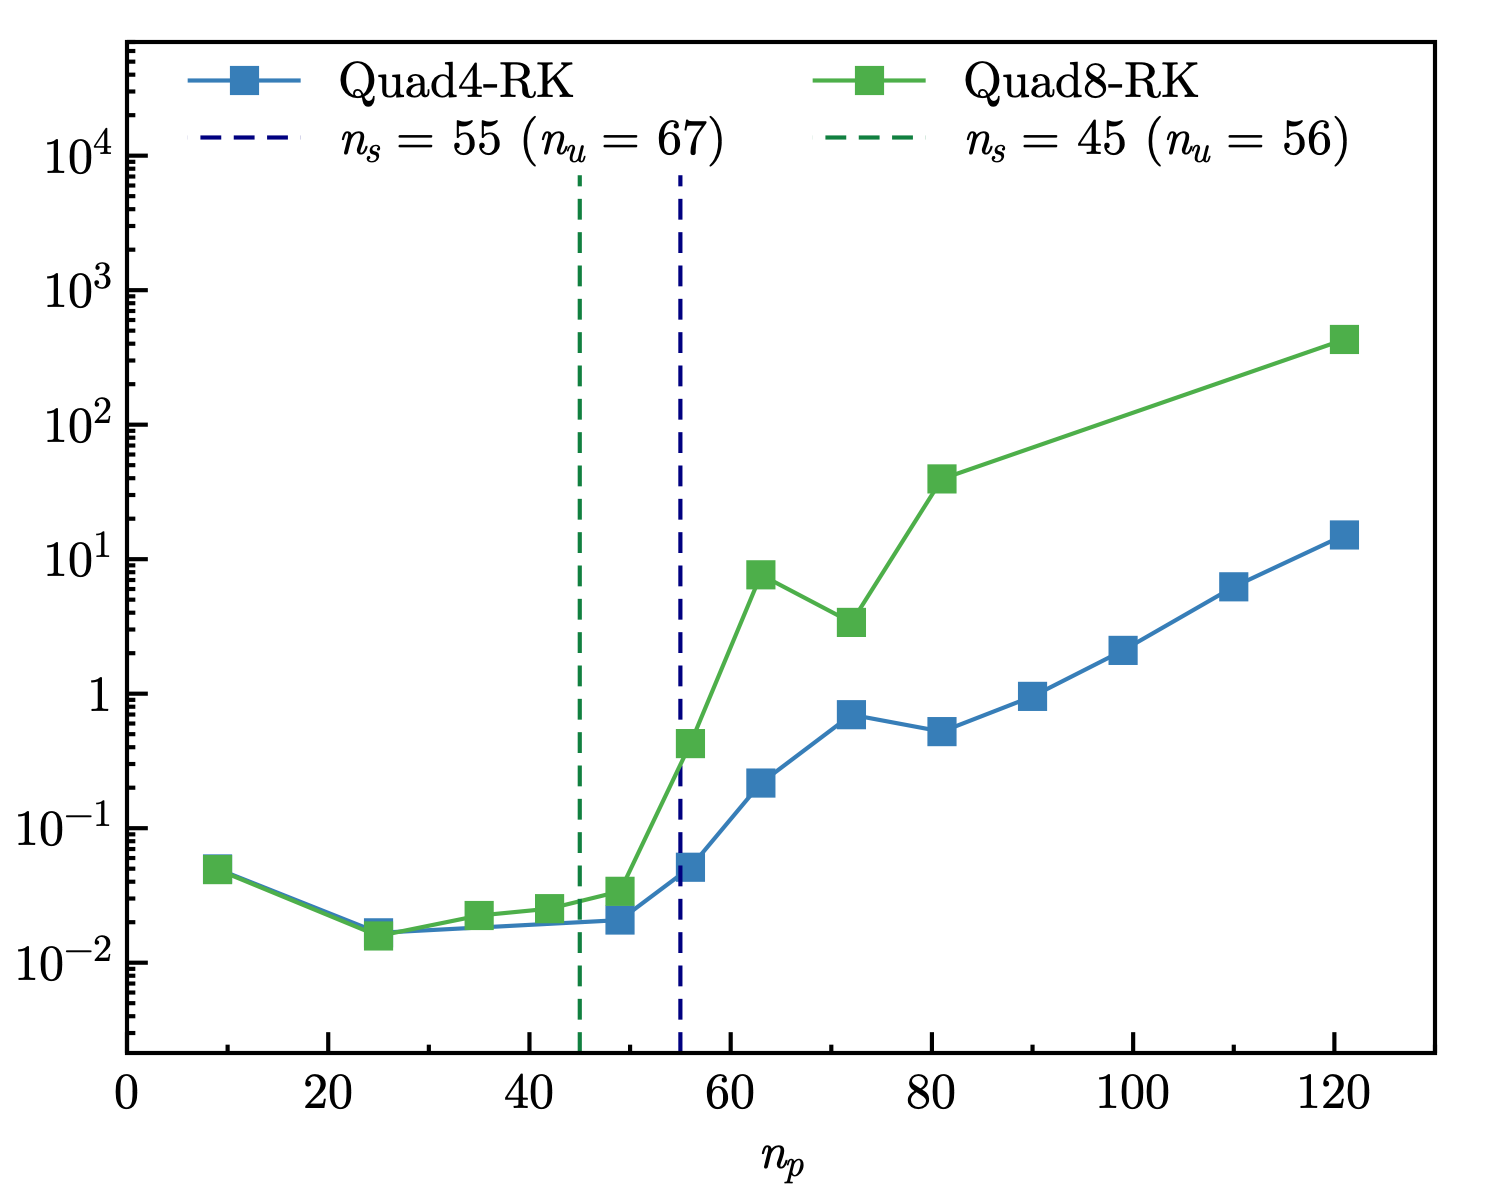
\includegraphics[width=0.45\textwidth]{png/cantilever_L2_p_4.png}}
    & \rotatebox{-90}{\parbox[b]{4cm}{Quad4: 85 nodes \\ Quad8: 80 nodes}} \\
      \raisebox{-0.85\height}{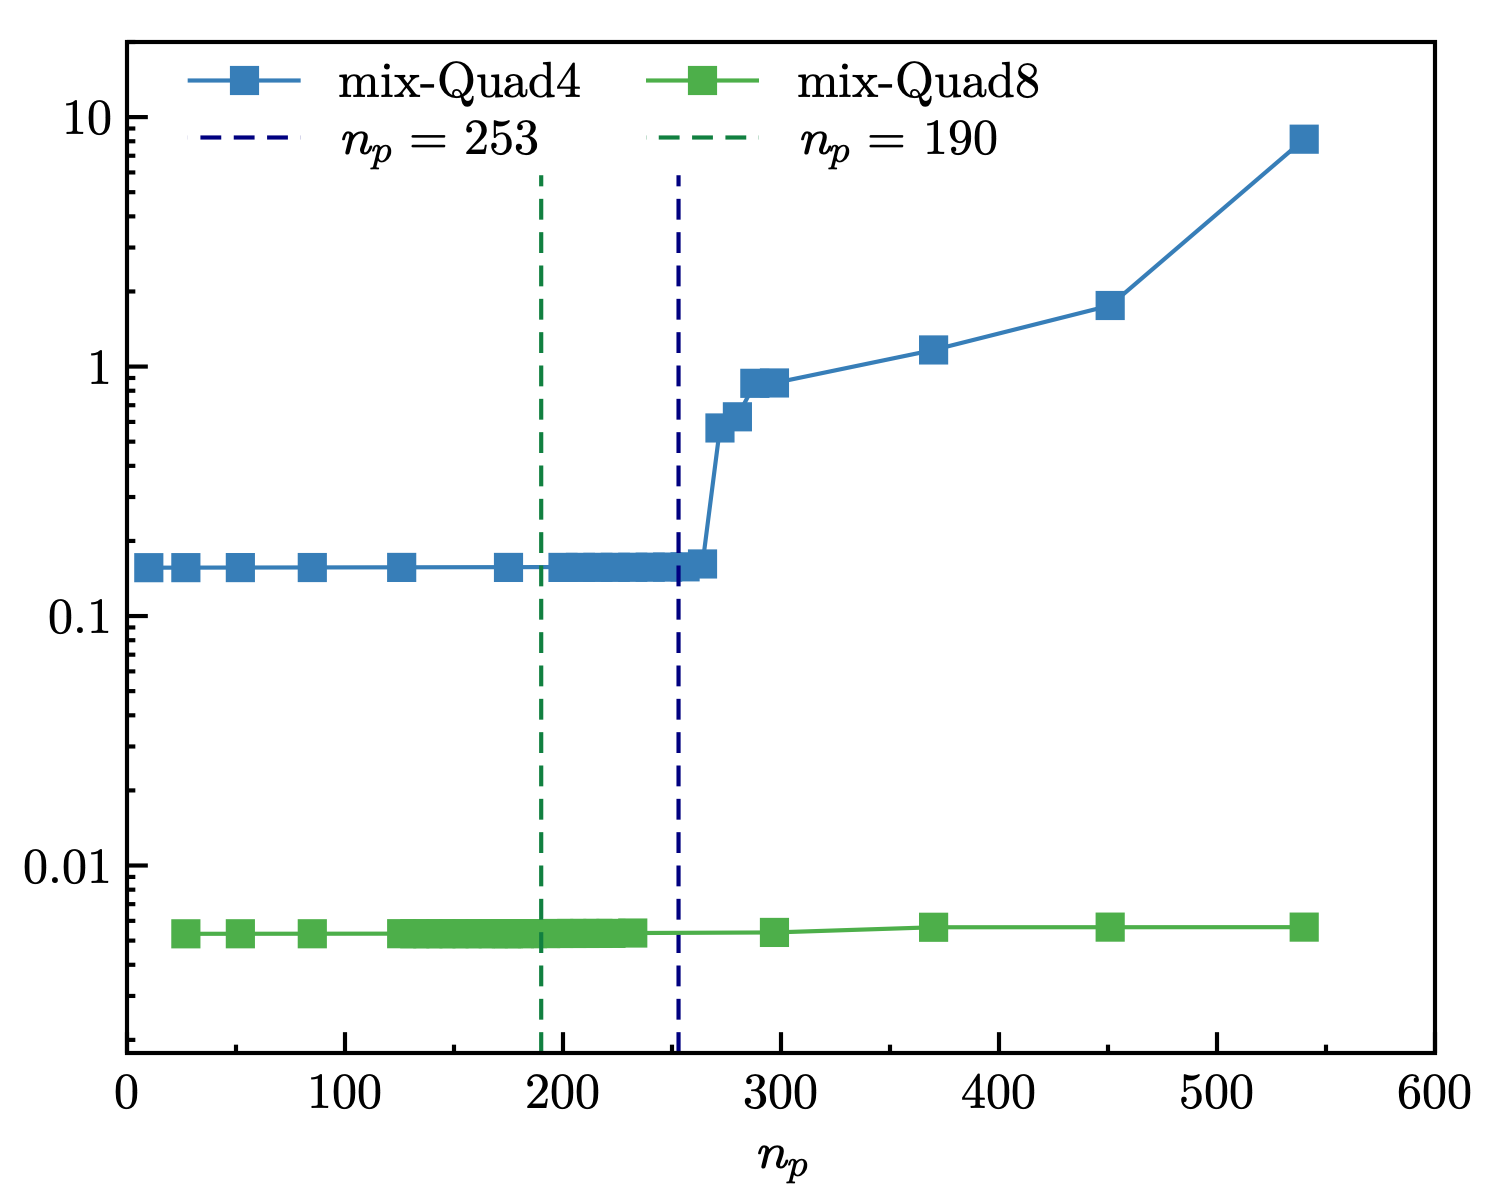
\includegraphics[width=0.45\textwidth]{png/cantilever_Hdev_8.png}}
    & \raisebox{-0.85\height}{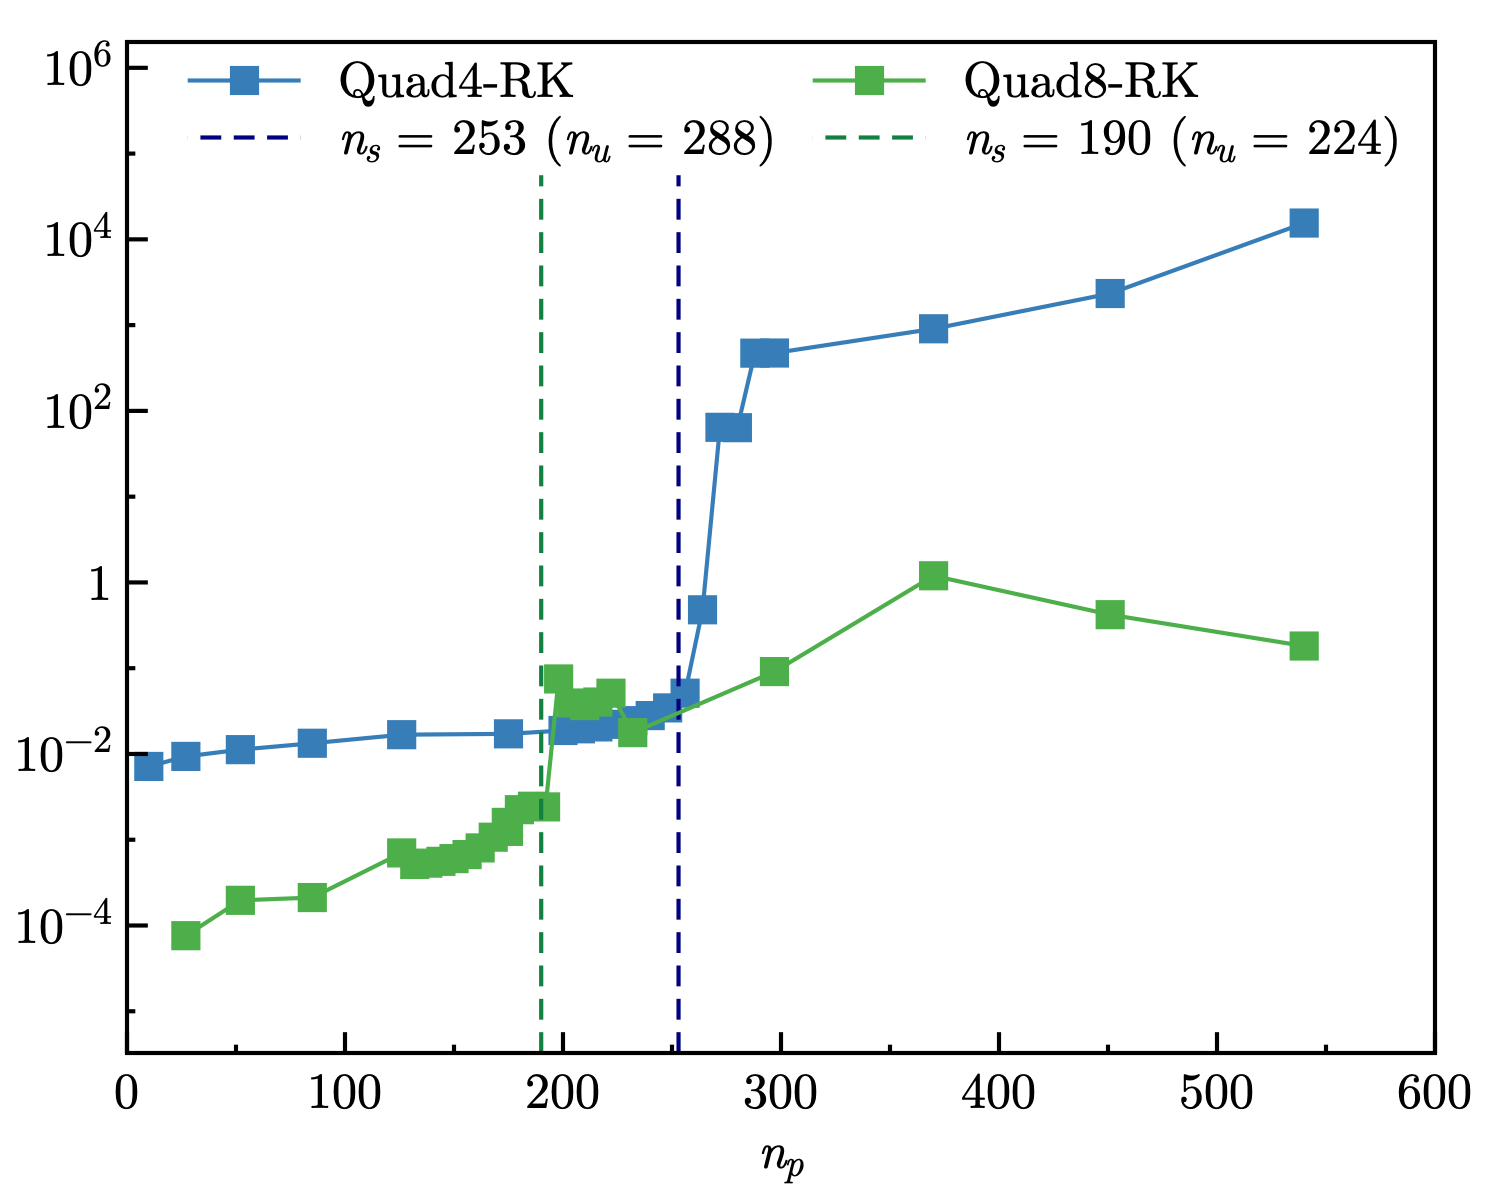
\includegraphics[width=0.45\textwidth]{png/cantilever_L2_p_8.png}}
    & \rotatebox{-90}{\parbox[b]{4cm}{Quad4: 297 nodes \\ Quad8: 288 nodes}} \\
      \raisebox{-0.85\height}{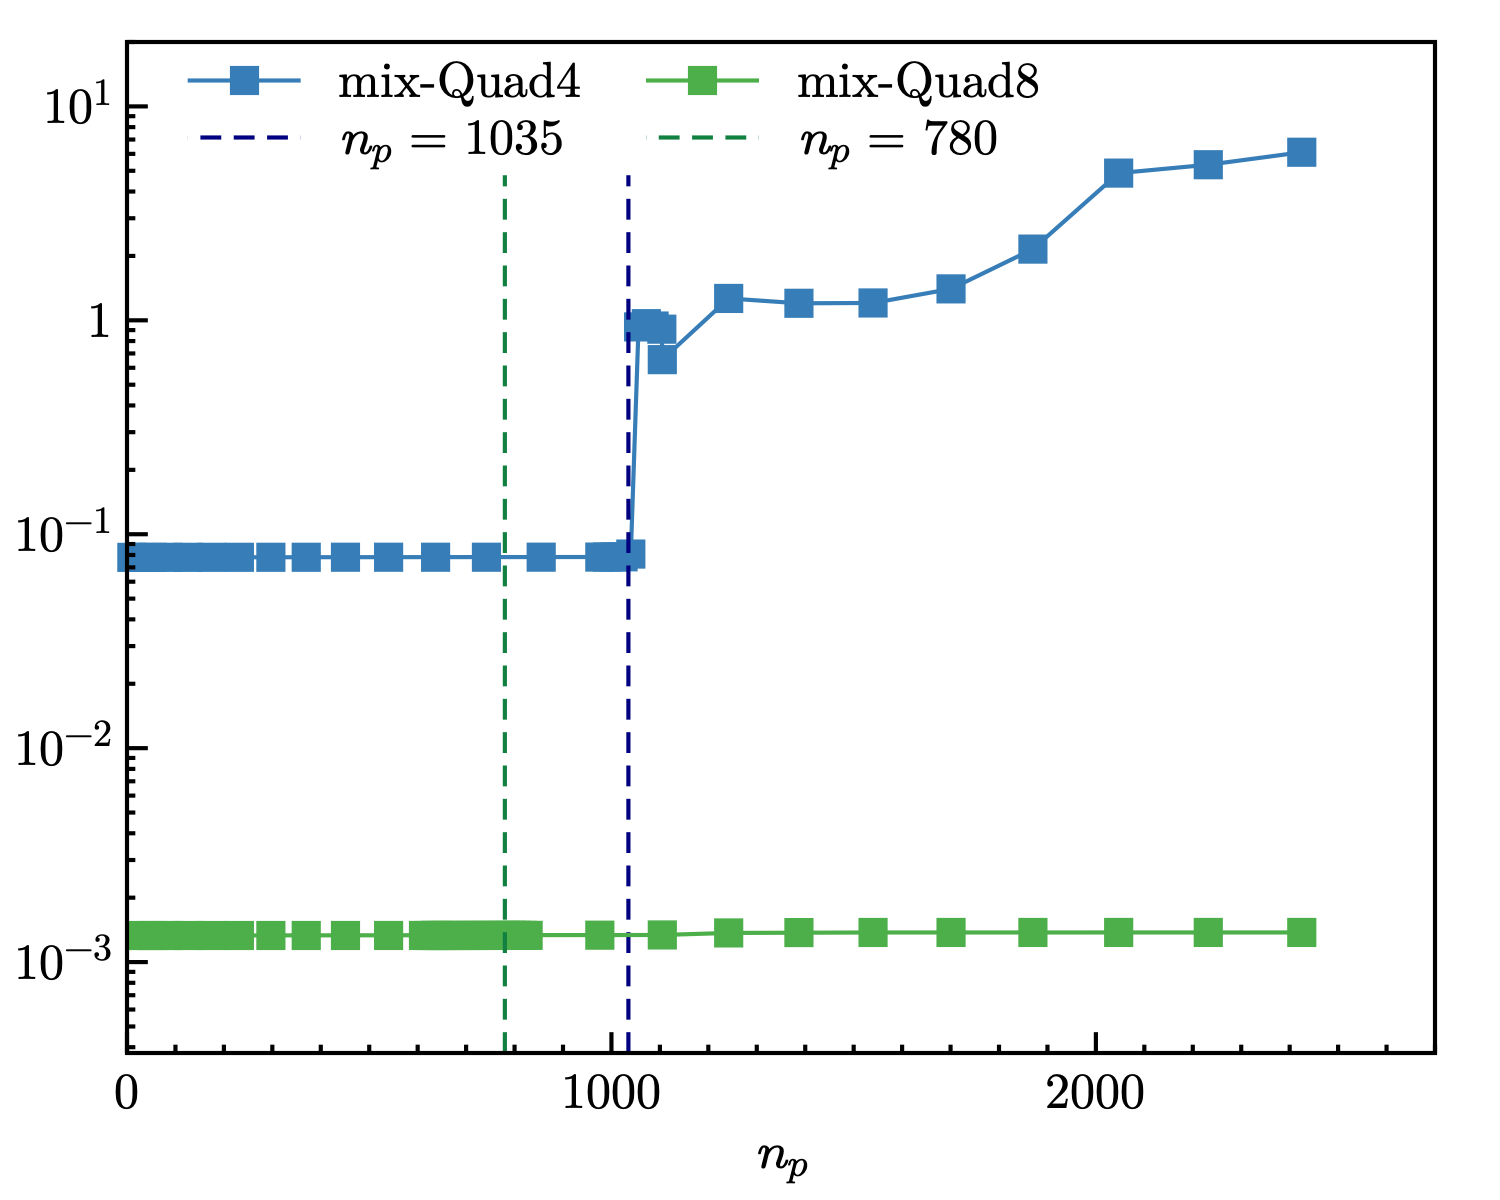
\includegraphics[width=0.45\textwidth]{png/cantilever_Hdev_16.png}}
    & \raisebox{-0.85\height}{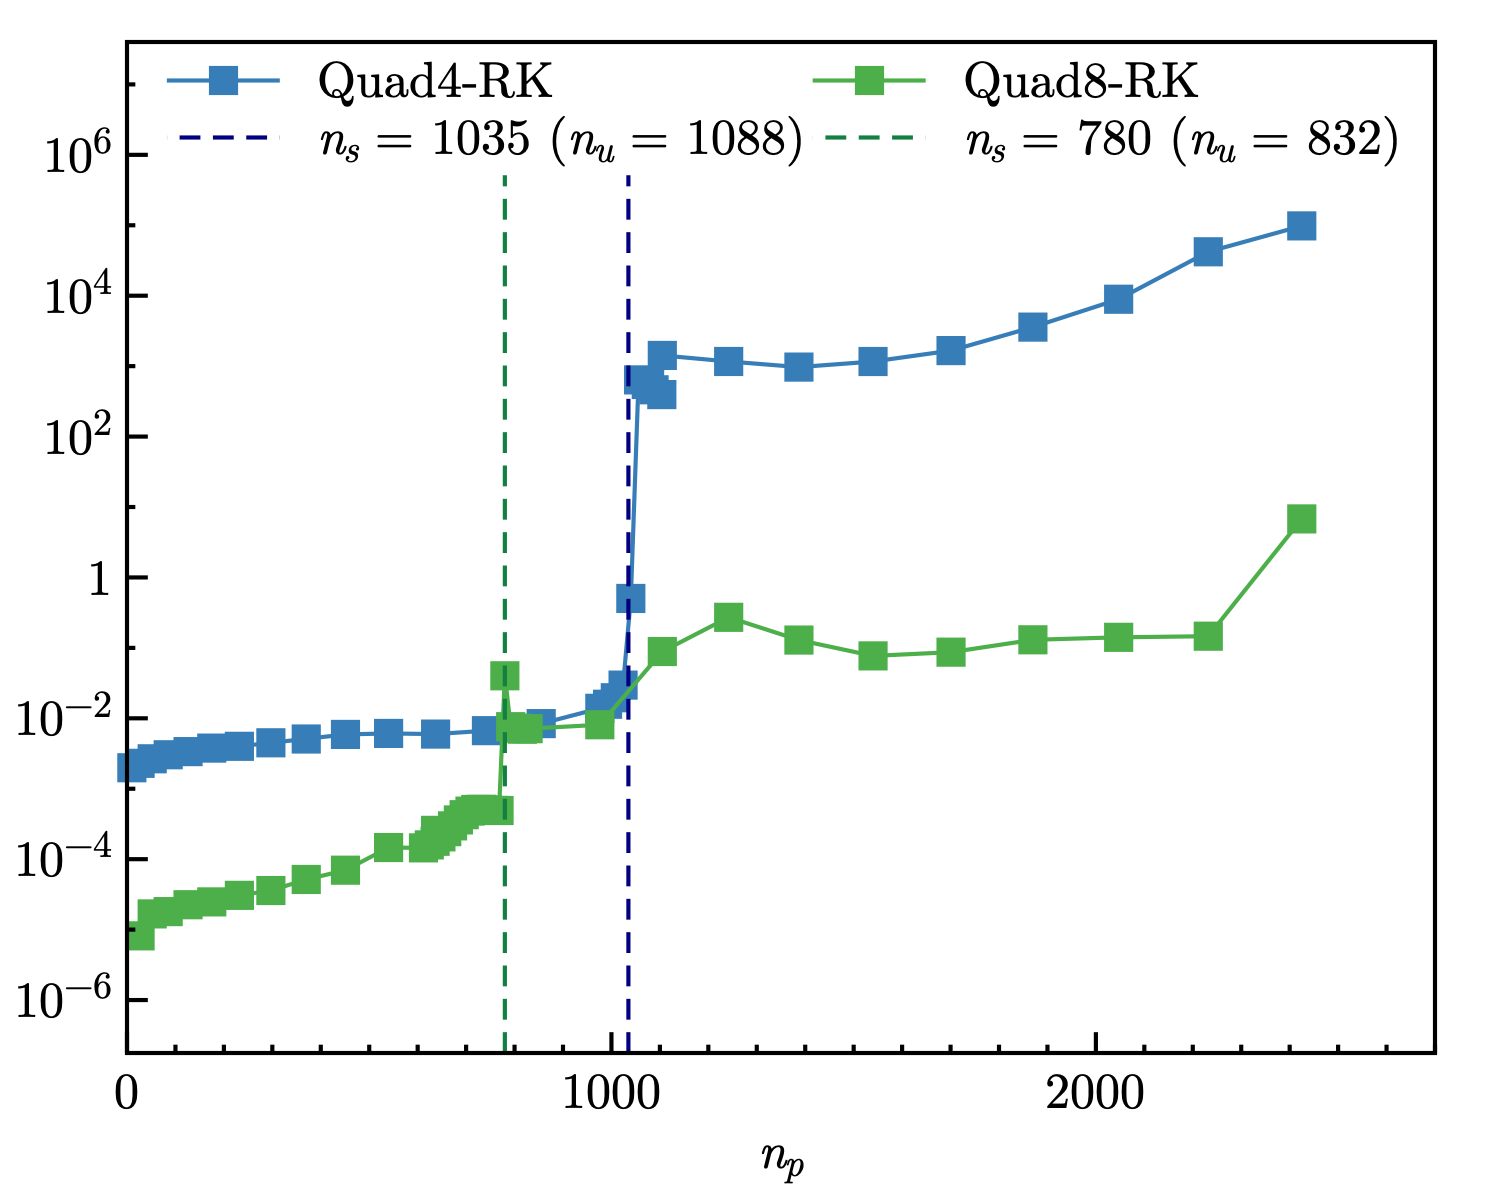
\includegraphics[width=0.45\textwidth]{png/cantilever_L2_p_16.png}}
    & \rotatebox{-90}{\parbox[b]{4cm}{Quad4: 1105 nodes \\ Quad8: 1088 nodes}} \\
      \raisebox{-0.85\height}{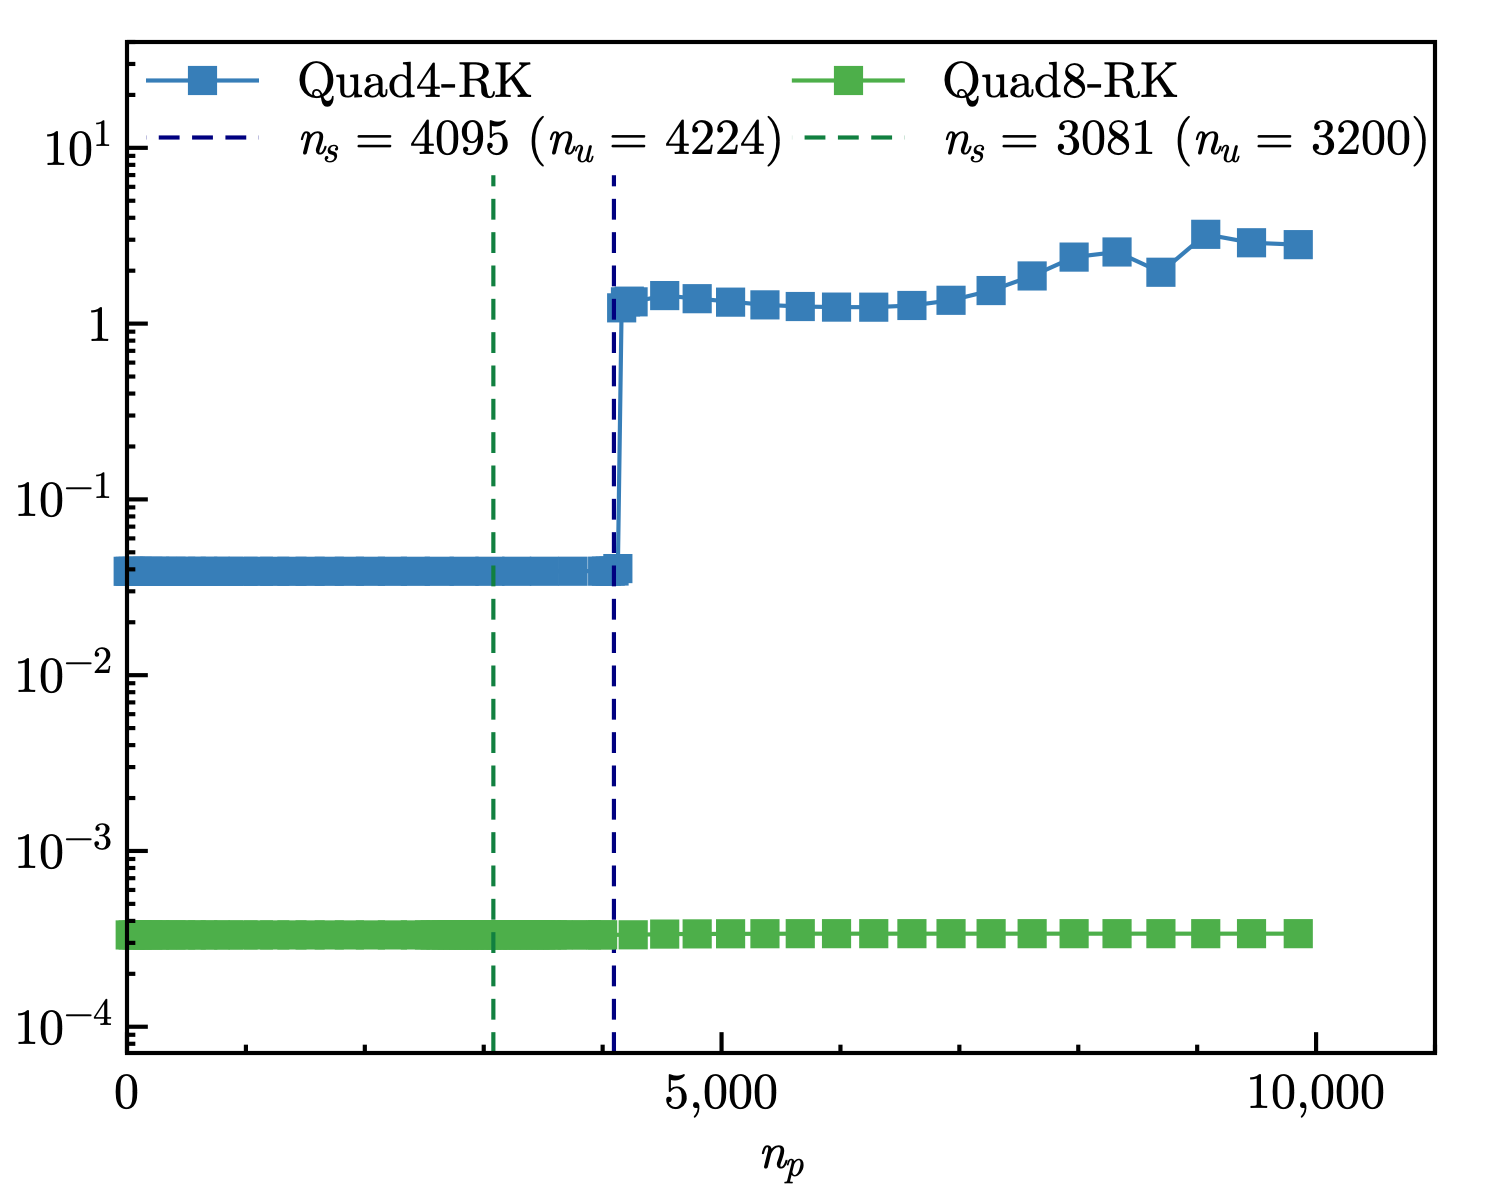
\includegraphics[width=0.45\textwidth]{png/cantilever_Hdev_32.png}}
    & \raisebox{-0.85\height}{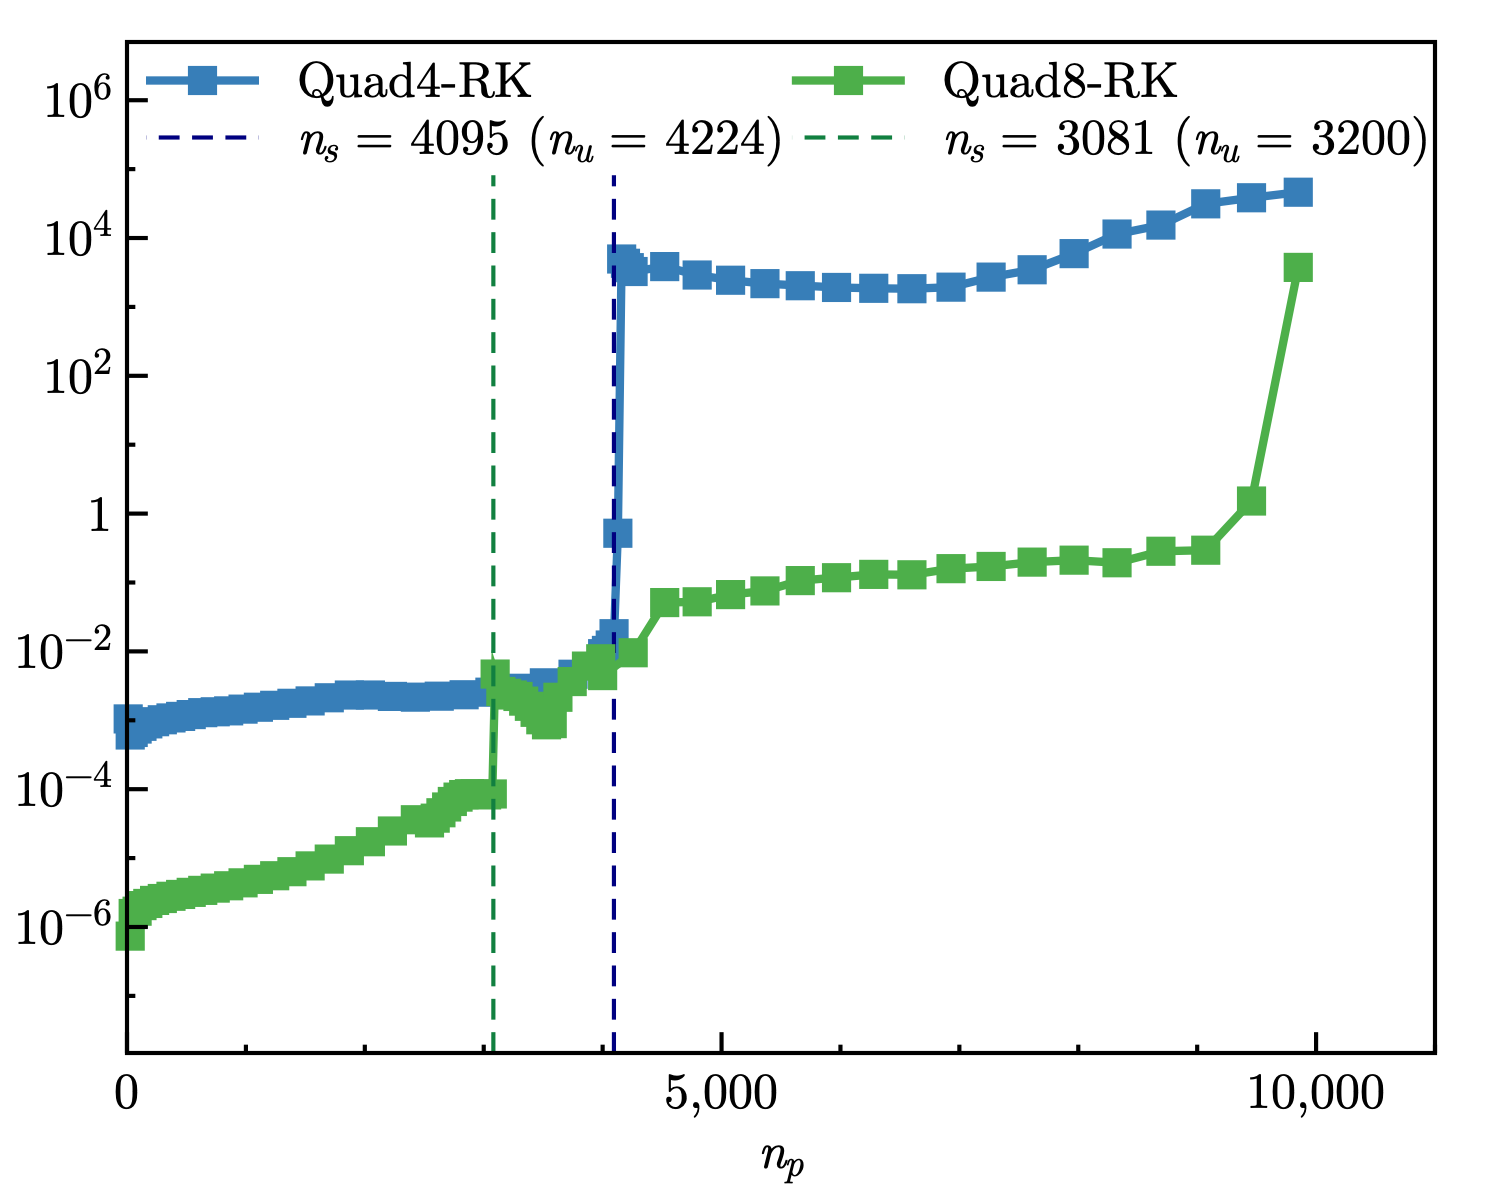
\includegraphics[width=0.45\textwidth]{png/cantilever_L2_p_32.png}}
    & \rotatebox{-90}{\parbox[b]{4cm}{Quad4: 4257 nodes \\ Quad8: 4224 nodes}} \\
    \end{tabular}
\end{subcaptiongroup}
\caption{}\label{cantilever_2}
\end{figure}

\begin{figure}[!ht]
\centering
% \includegraphics[width=\textwidth]{png/cantilever4.png}
\caption{Contour plots of cantilever beam problem}\label{cantilever_contour}
\end{figure}

\subsection{Plate with hole problem}

\begin{figure}[!ht]
\centering
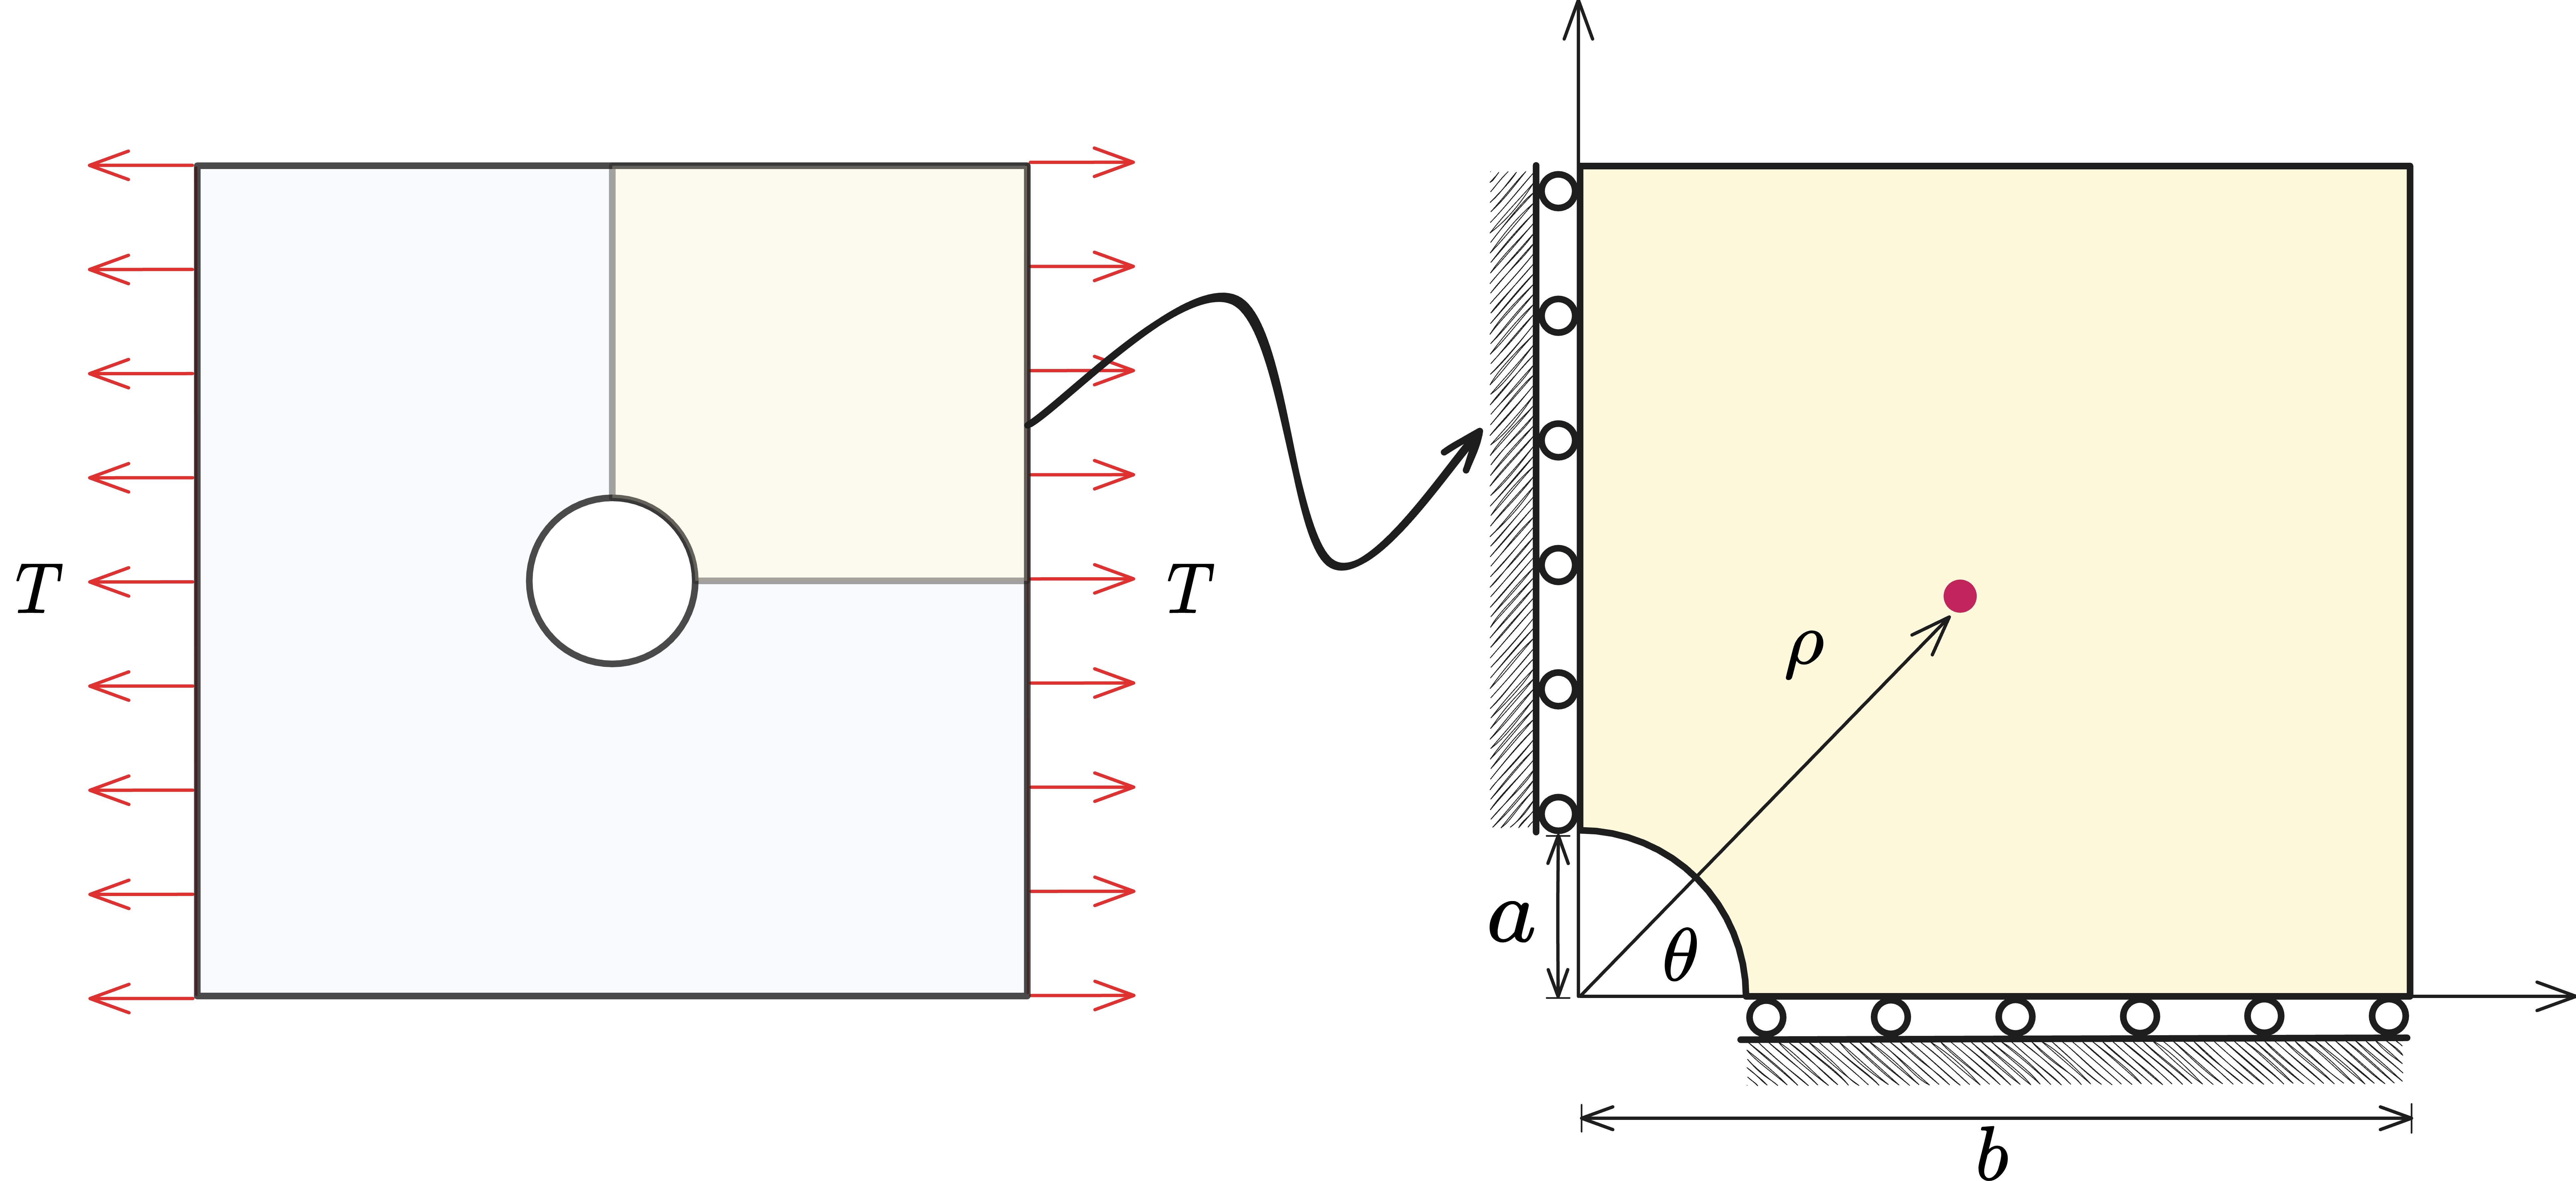
\includegraphics[width=0.8\textwidth]{png/plate_with_hole_model.png}
\caption{Illustration of plate with hole problem}\label{plate_with_hole_1}
\end{figure}

\begin{figure}[!ht]
\centering
\begin{subcaptiongroup}
    \begin{tabular}{c@{\hspace{0pt}}c@{\hspace{0pt}}c}
      $\Vert \boldsymbol u - \boldsymbol u_h \Vert_V$ & $\Vert p - p_h \Vert_Q$ & \\
      \raisebox{-0.7\height}{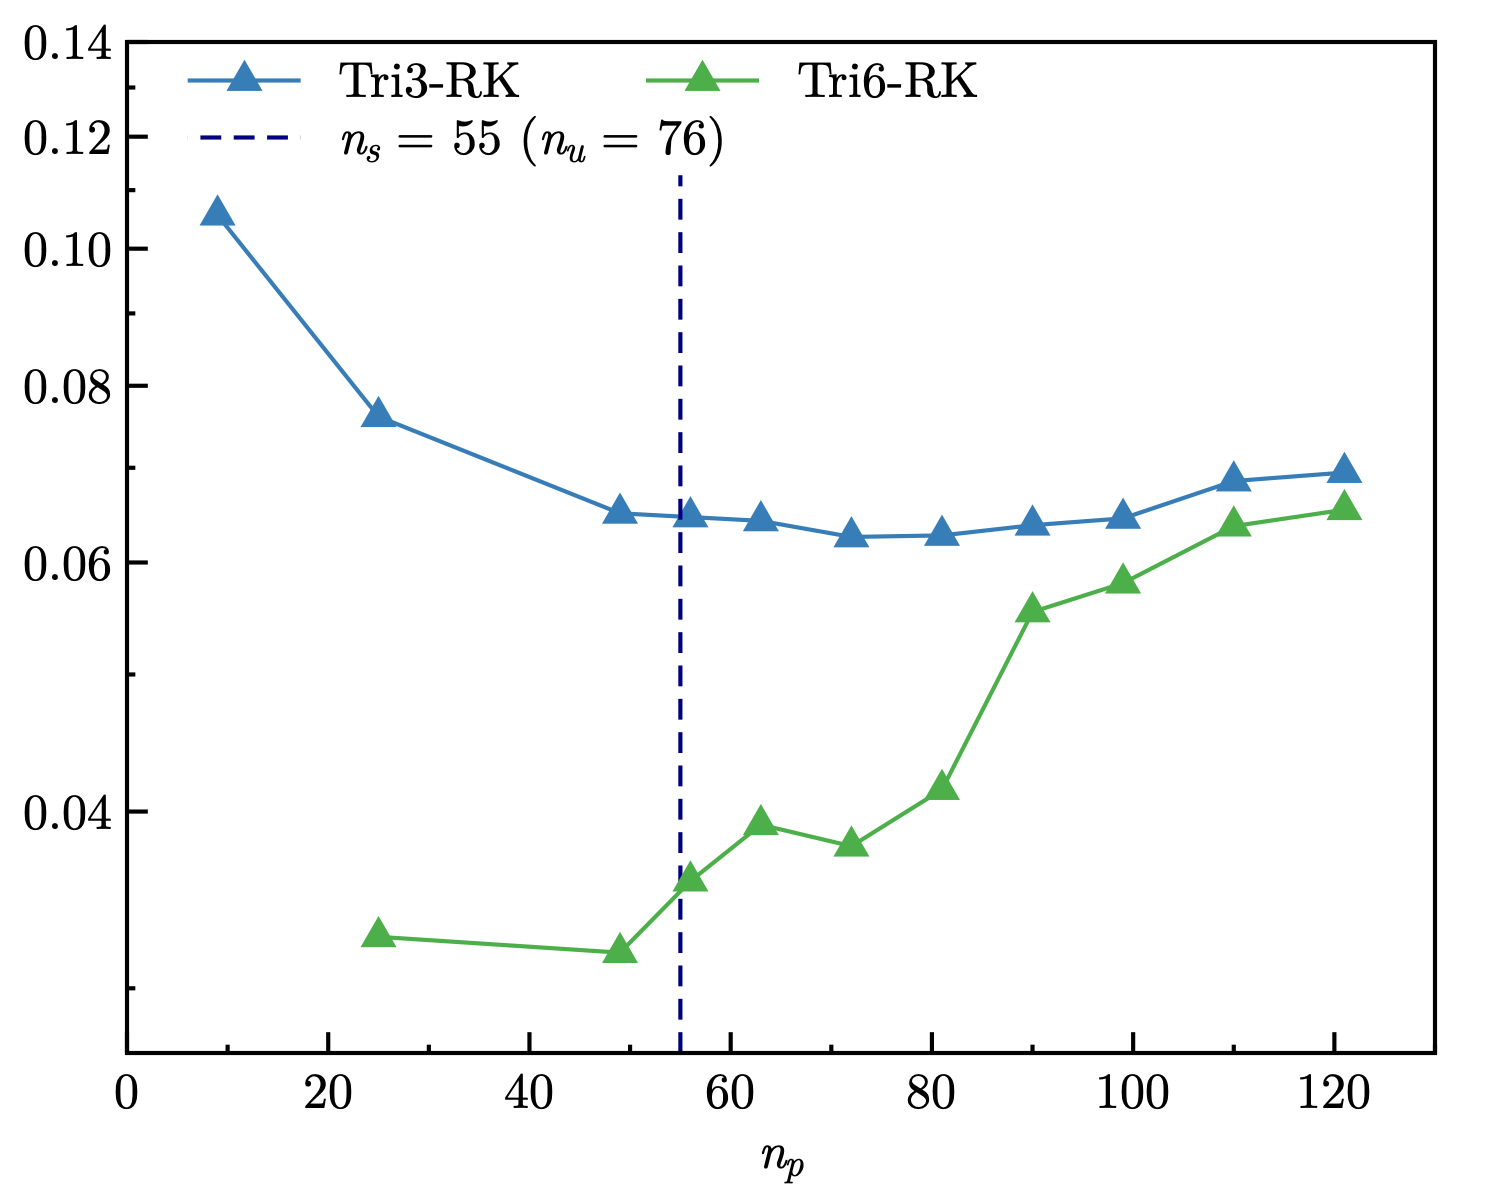
\includegraphics[width=0.45\textwidth]{png/plate_Hdev_4.png}}
    & \raisebox{-0.7\height}{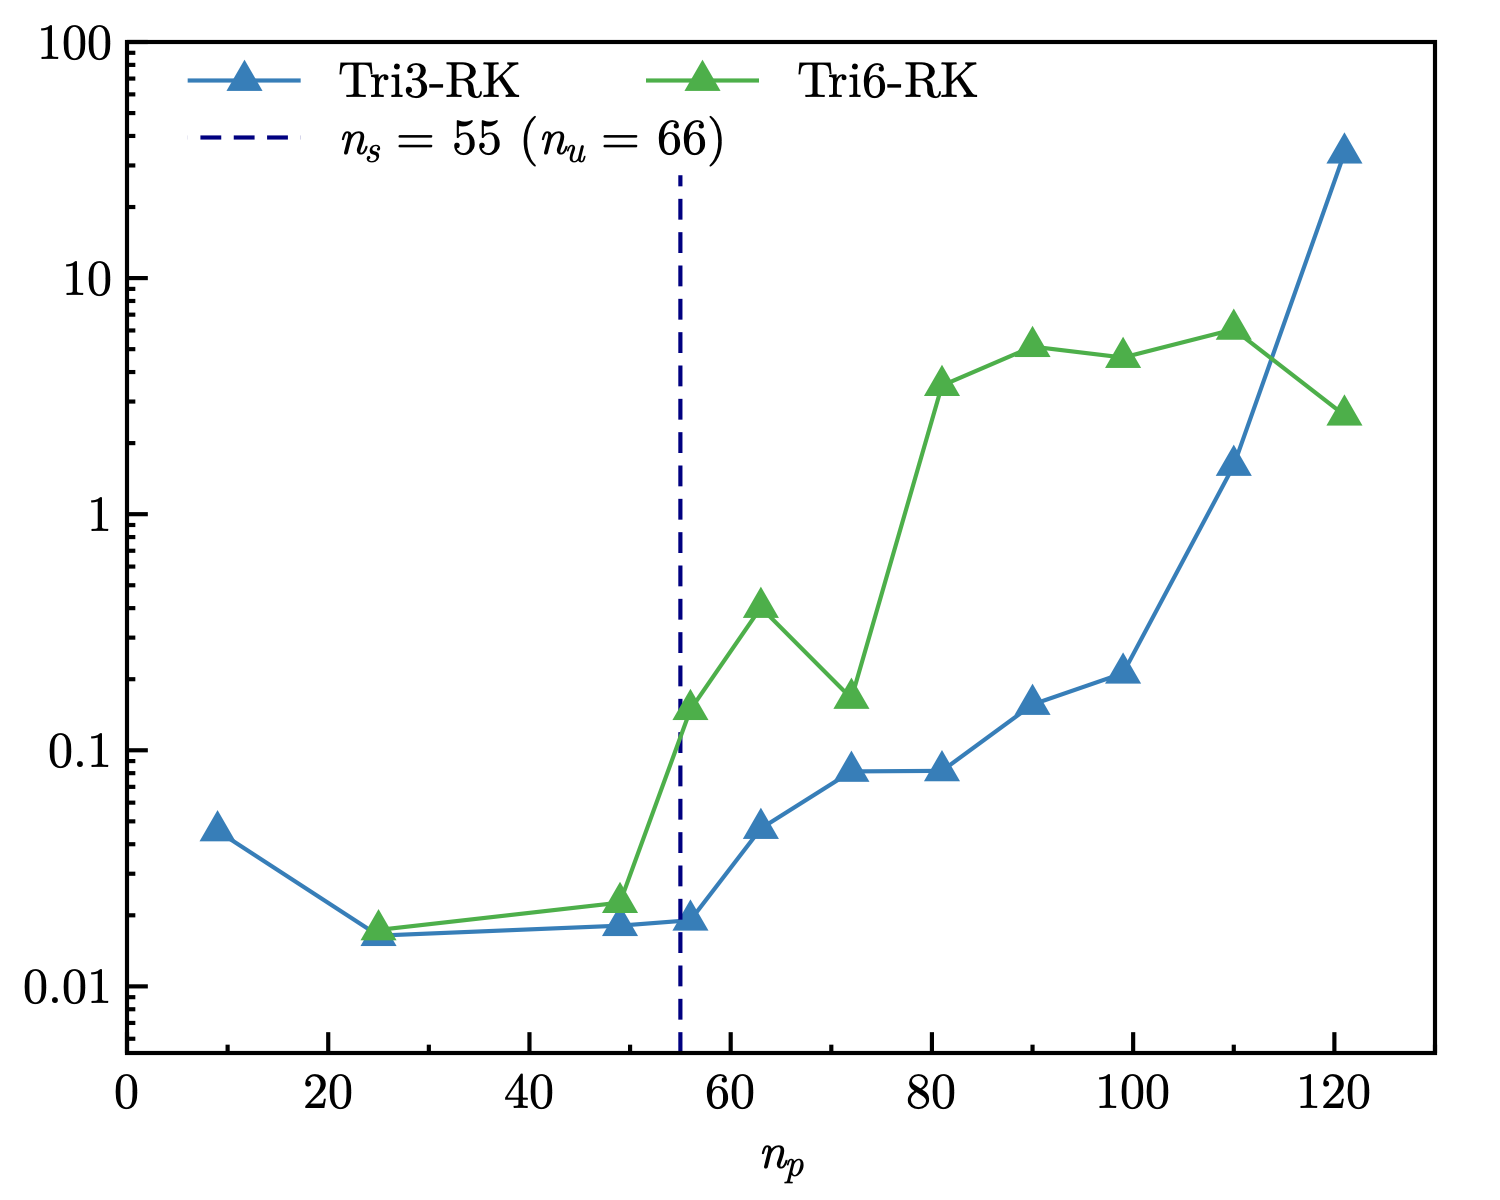
\includegraphics[width=0.45\textwidth]{png/plate_L2_p_4.png}}
    & \rotatebox{-90}{81 nodes} \\
      \raisebox{-0.7\height}{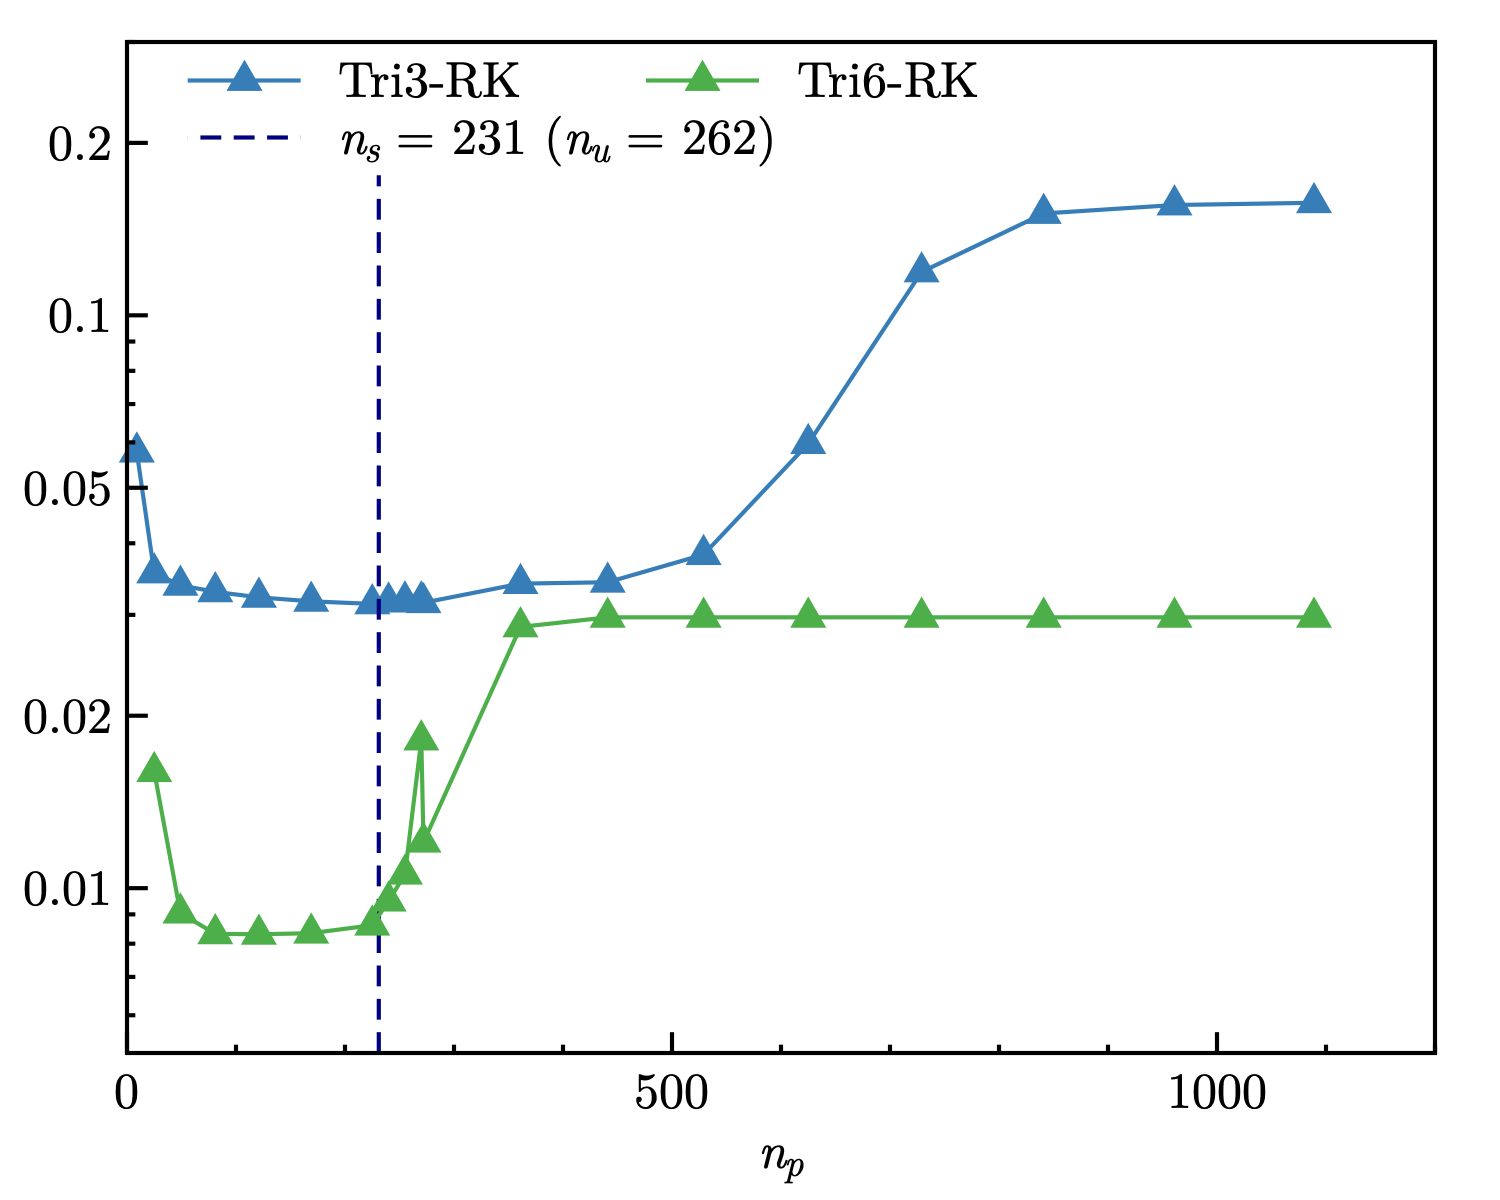
\includegraphics[width=0.45\textwidth]{png/plate_Hdev_8.png}}
    & \raisebox{-0.7\height}{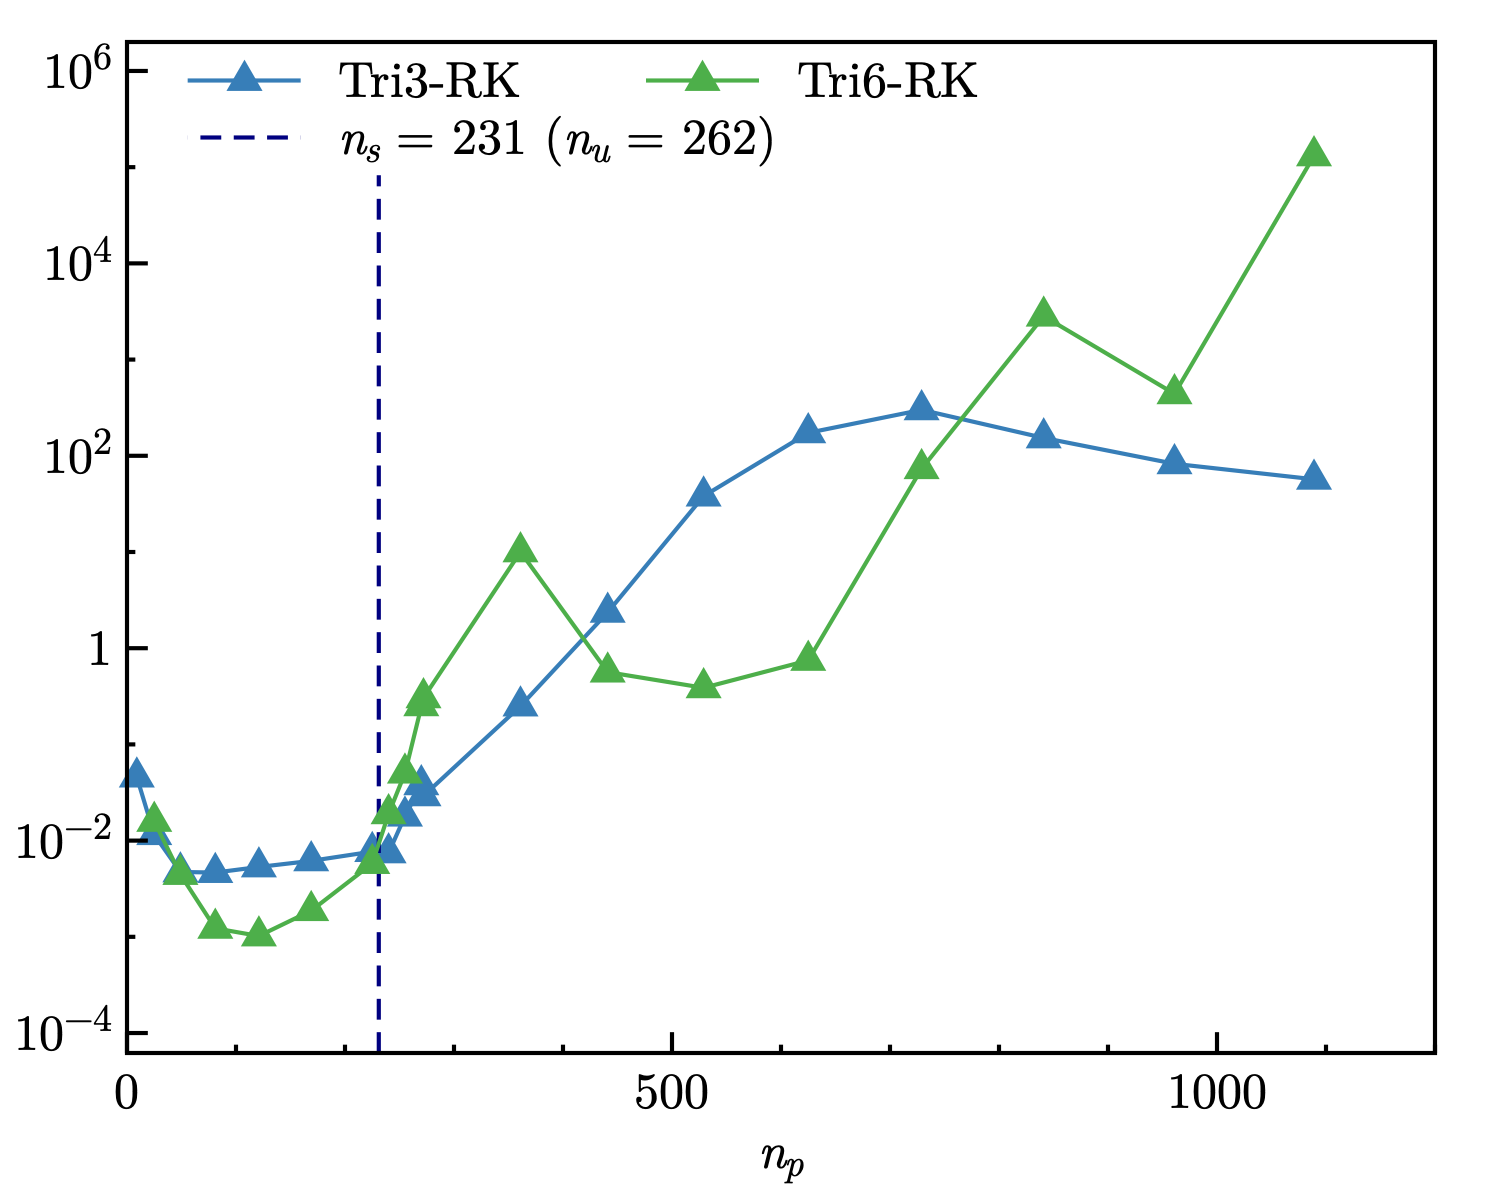
\includegraphics[width=0.45\textwidth]{png/plate_L2_p_8.png}}
    & \rotatebox{-90}{289 nodes} \\
      \raisebox{-0.7\height}{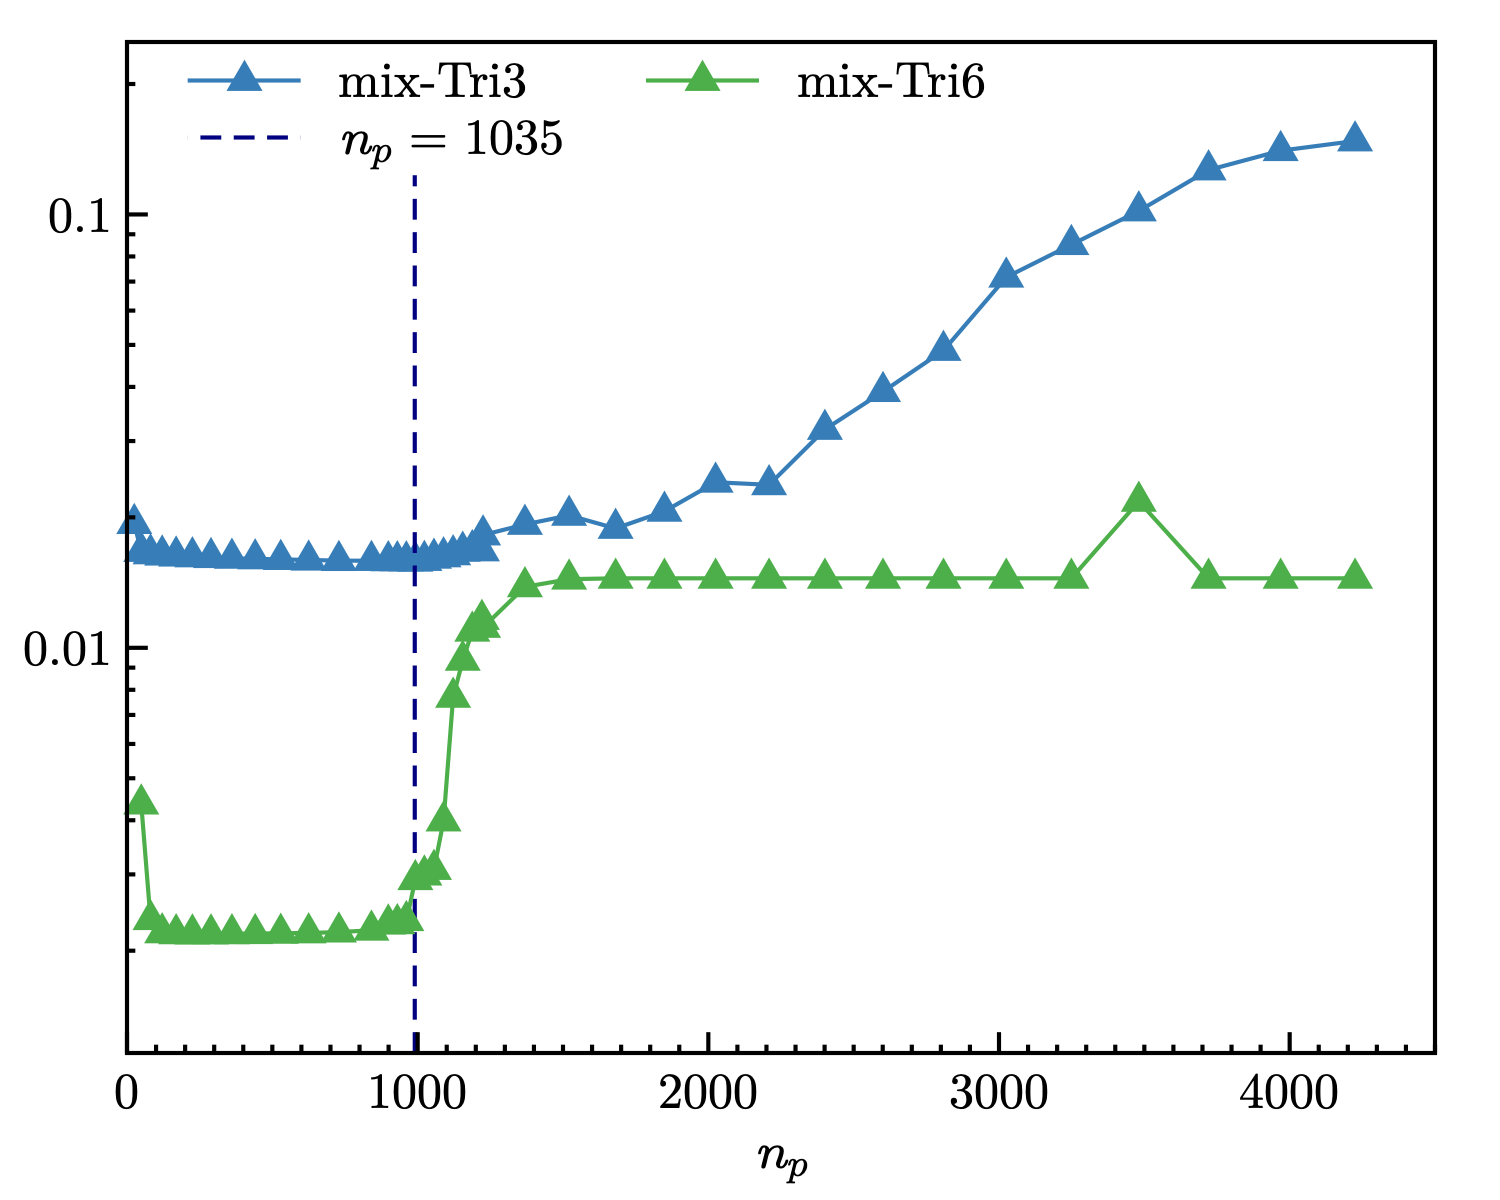
\includegraphics[width=0.45\textwidth]{png/plate_Hdev_16.png}}
    & \raisebox{-0.7\height}{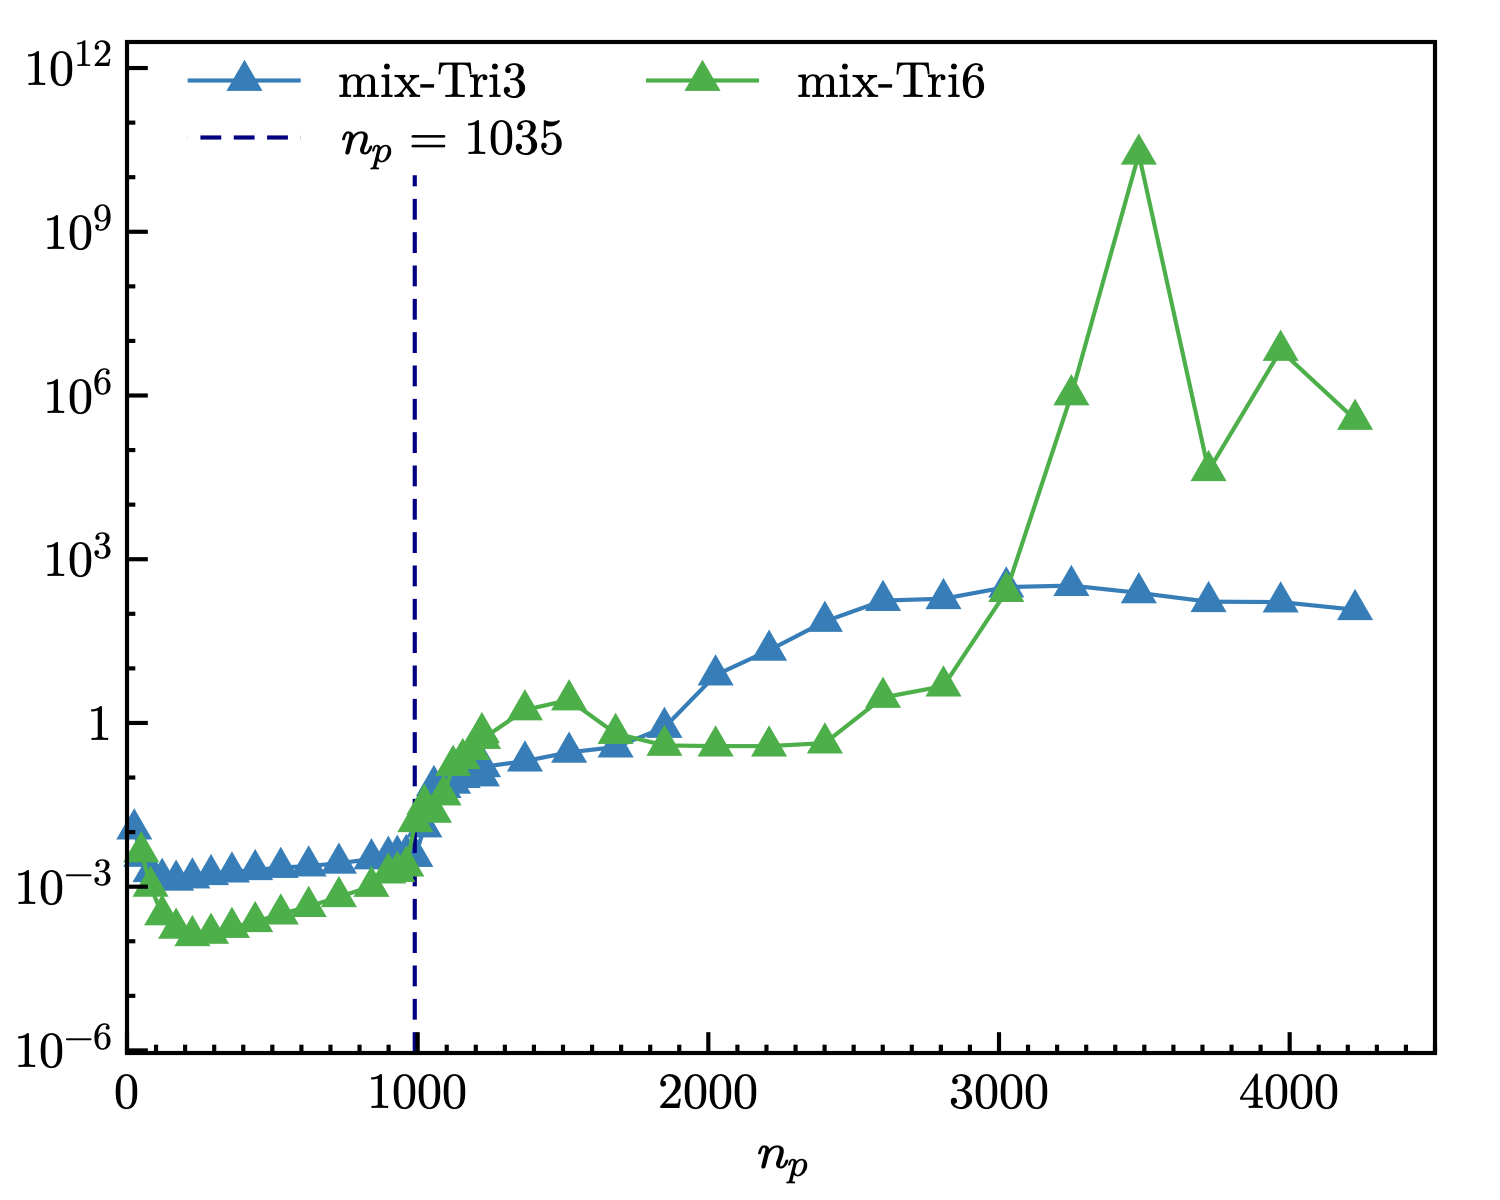
\includegraphics[width=0.45\textwidth]{png/plate_L2_p_16.png}}
    & \rotatebox{-90}{1089 nodes} \\
      \raisebox{-0.7\height}{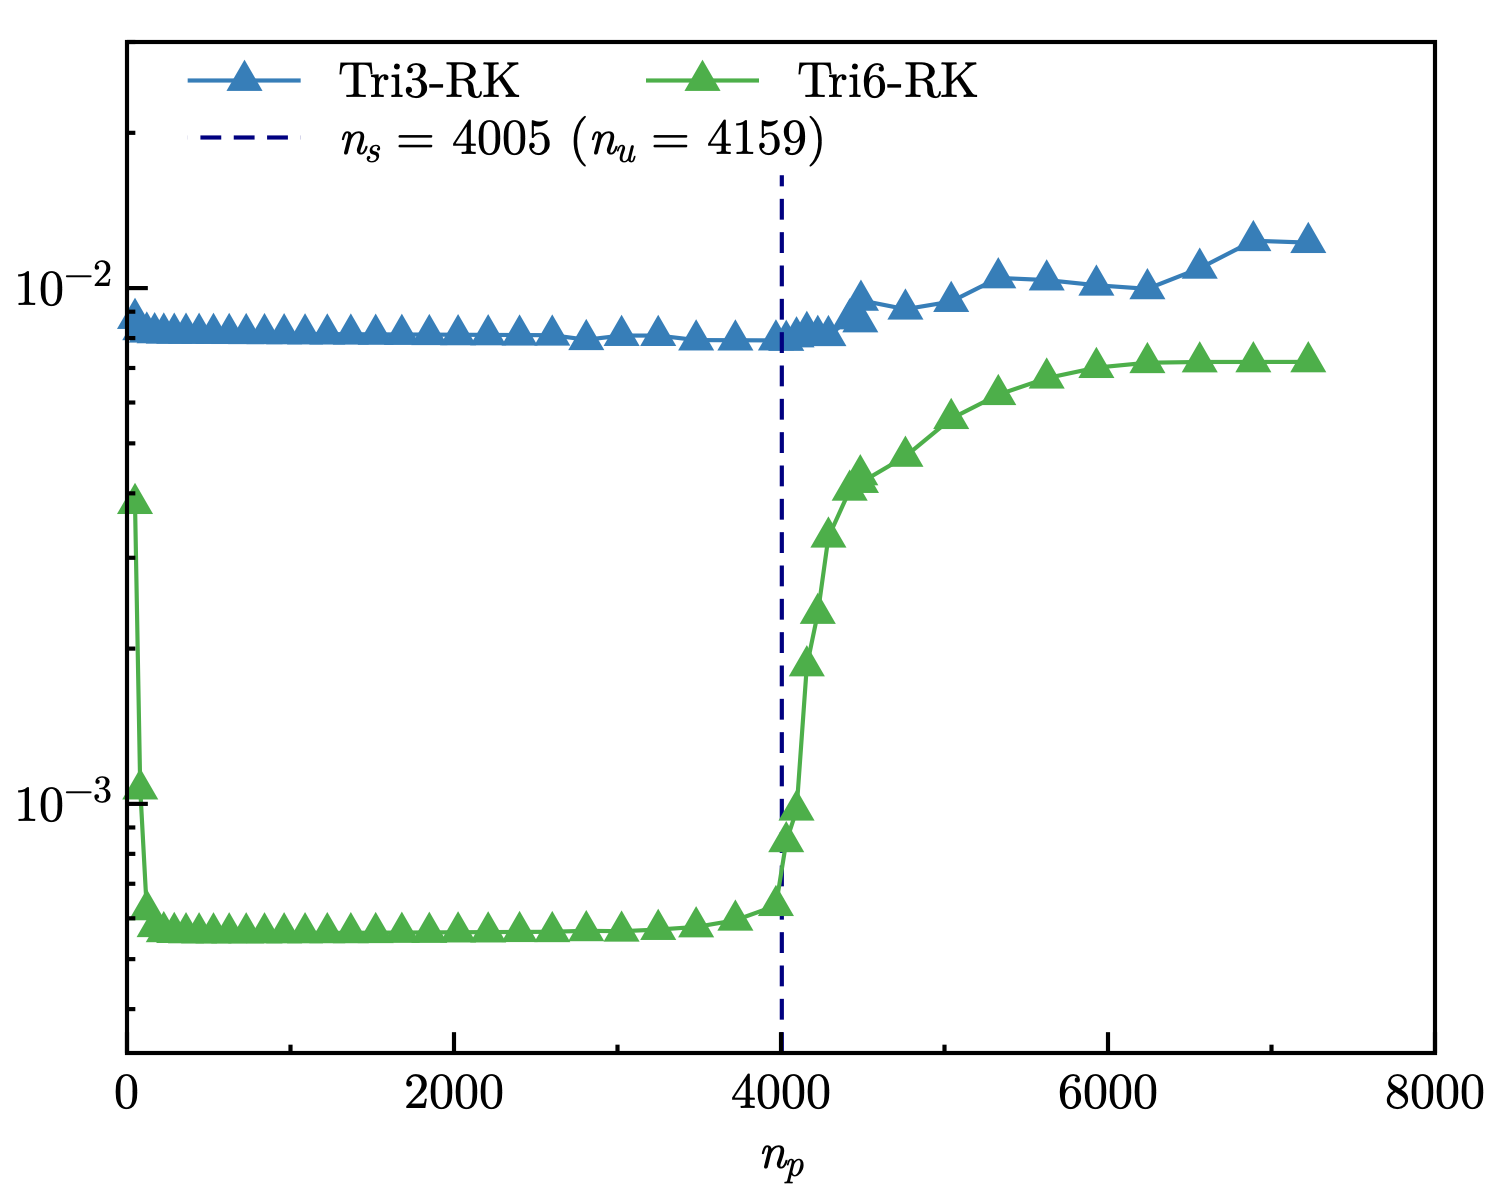
\includegraphics[width=0.45\textwidth]{png/plate_Hdev_32.png}}
    & \raisebox{-0.7\height}{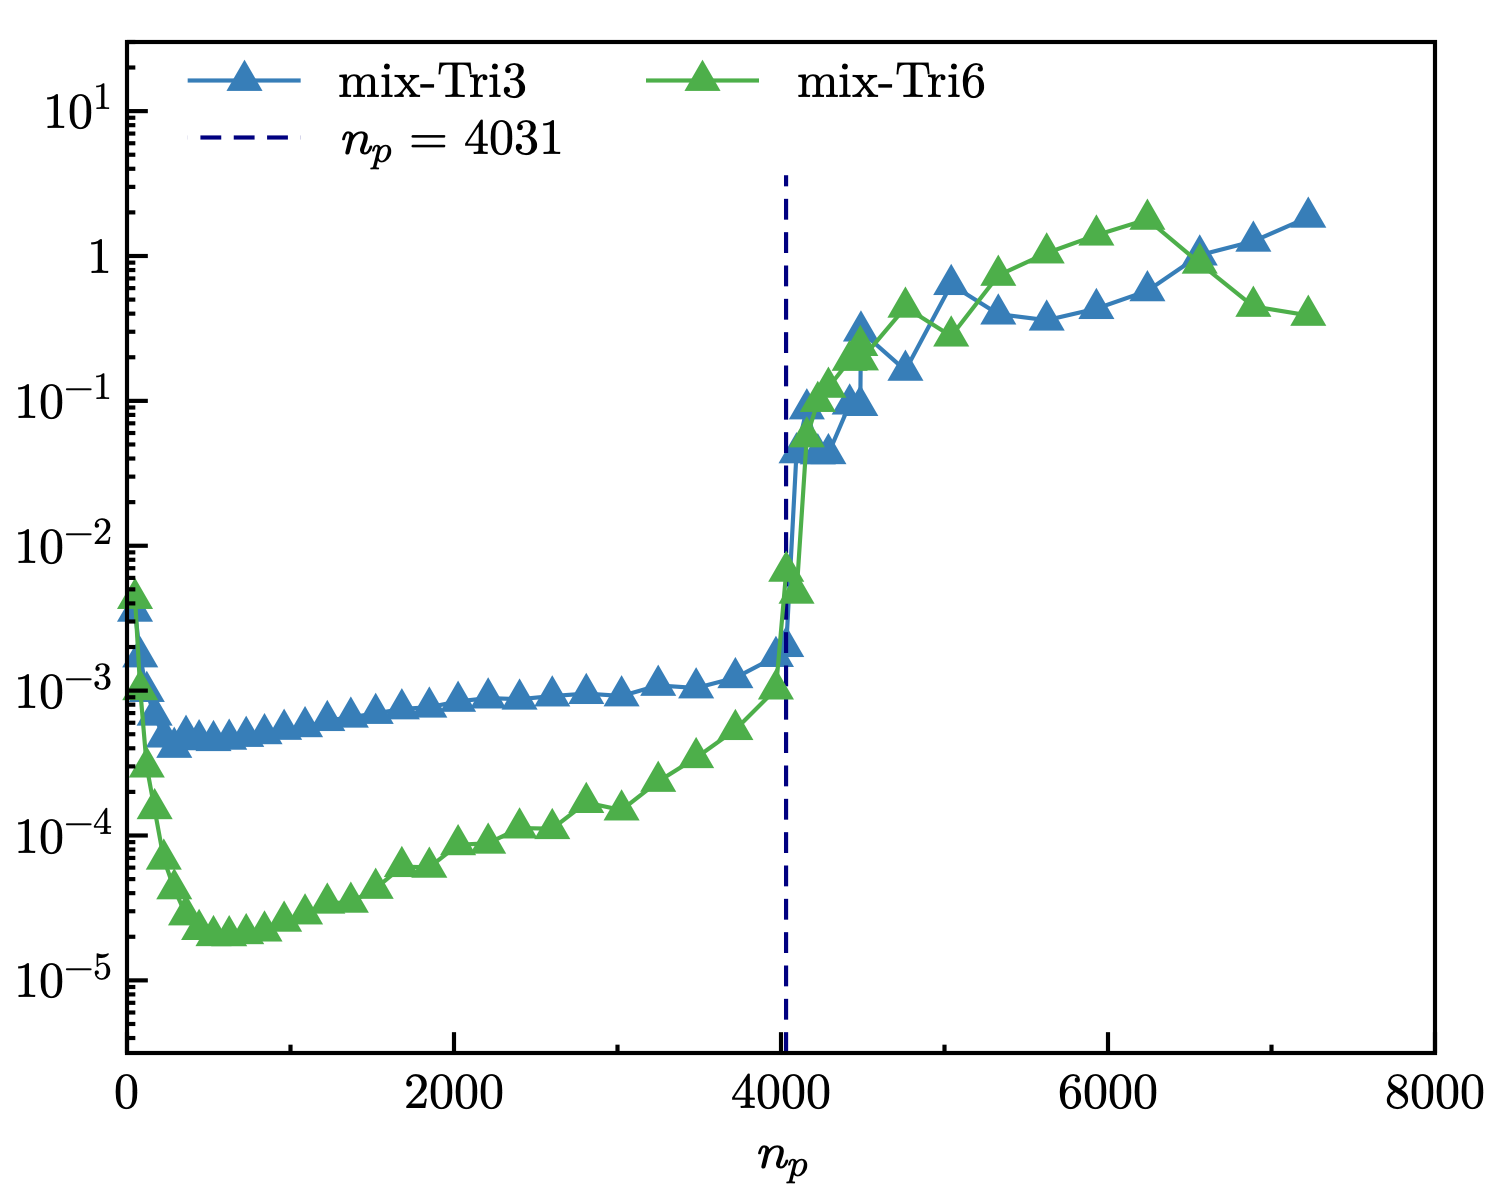
\includegraphics[width=0.45\textwidth]{png/plate_L2_p_32.png}}
    & \rotatebox{-90}{4225 nodes} \\
    \end{tabular}
\end{subcaptiongroup}
\caption{}\label{plate_with_hole_2}
\end{figure}

\begin{figure}[!ht]
\centering
% \includegraphics[width=\textwidth]{png/cantilever4.png}
\caption{Contour plots of cantilever beam problem}\label{plate_with_hole_contour}
\end{figure}
\begin{figure}[!ht]
\centering
%\includegraphics[width=0.7\textwidth]{png/cook2.png}
\caption{Convergence comparison of cook membrane problem}\label{cook_convergence}
\end{figure}

\begin{figure}[!ht]
\centering
% \includegraphics[width=\textwidth]{png/cook3.png}
\caption{Contour plots of cook membrane problem}\label{cook_contour}
\end{figure}

\subsection{Cook membrane problem}

\begin{figure}[!ht]
\centering
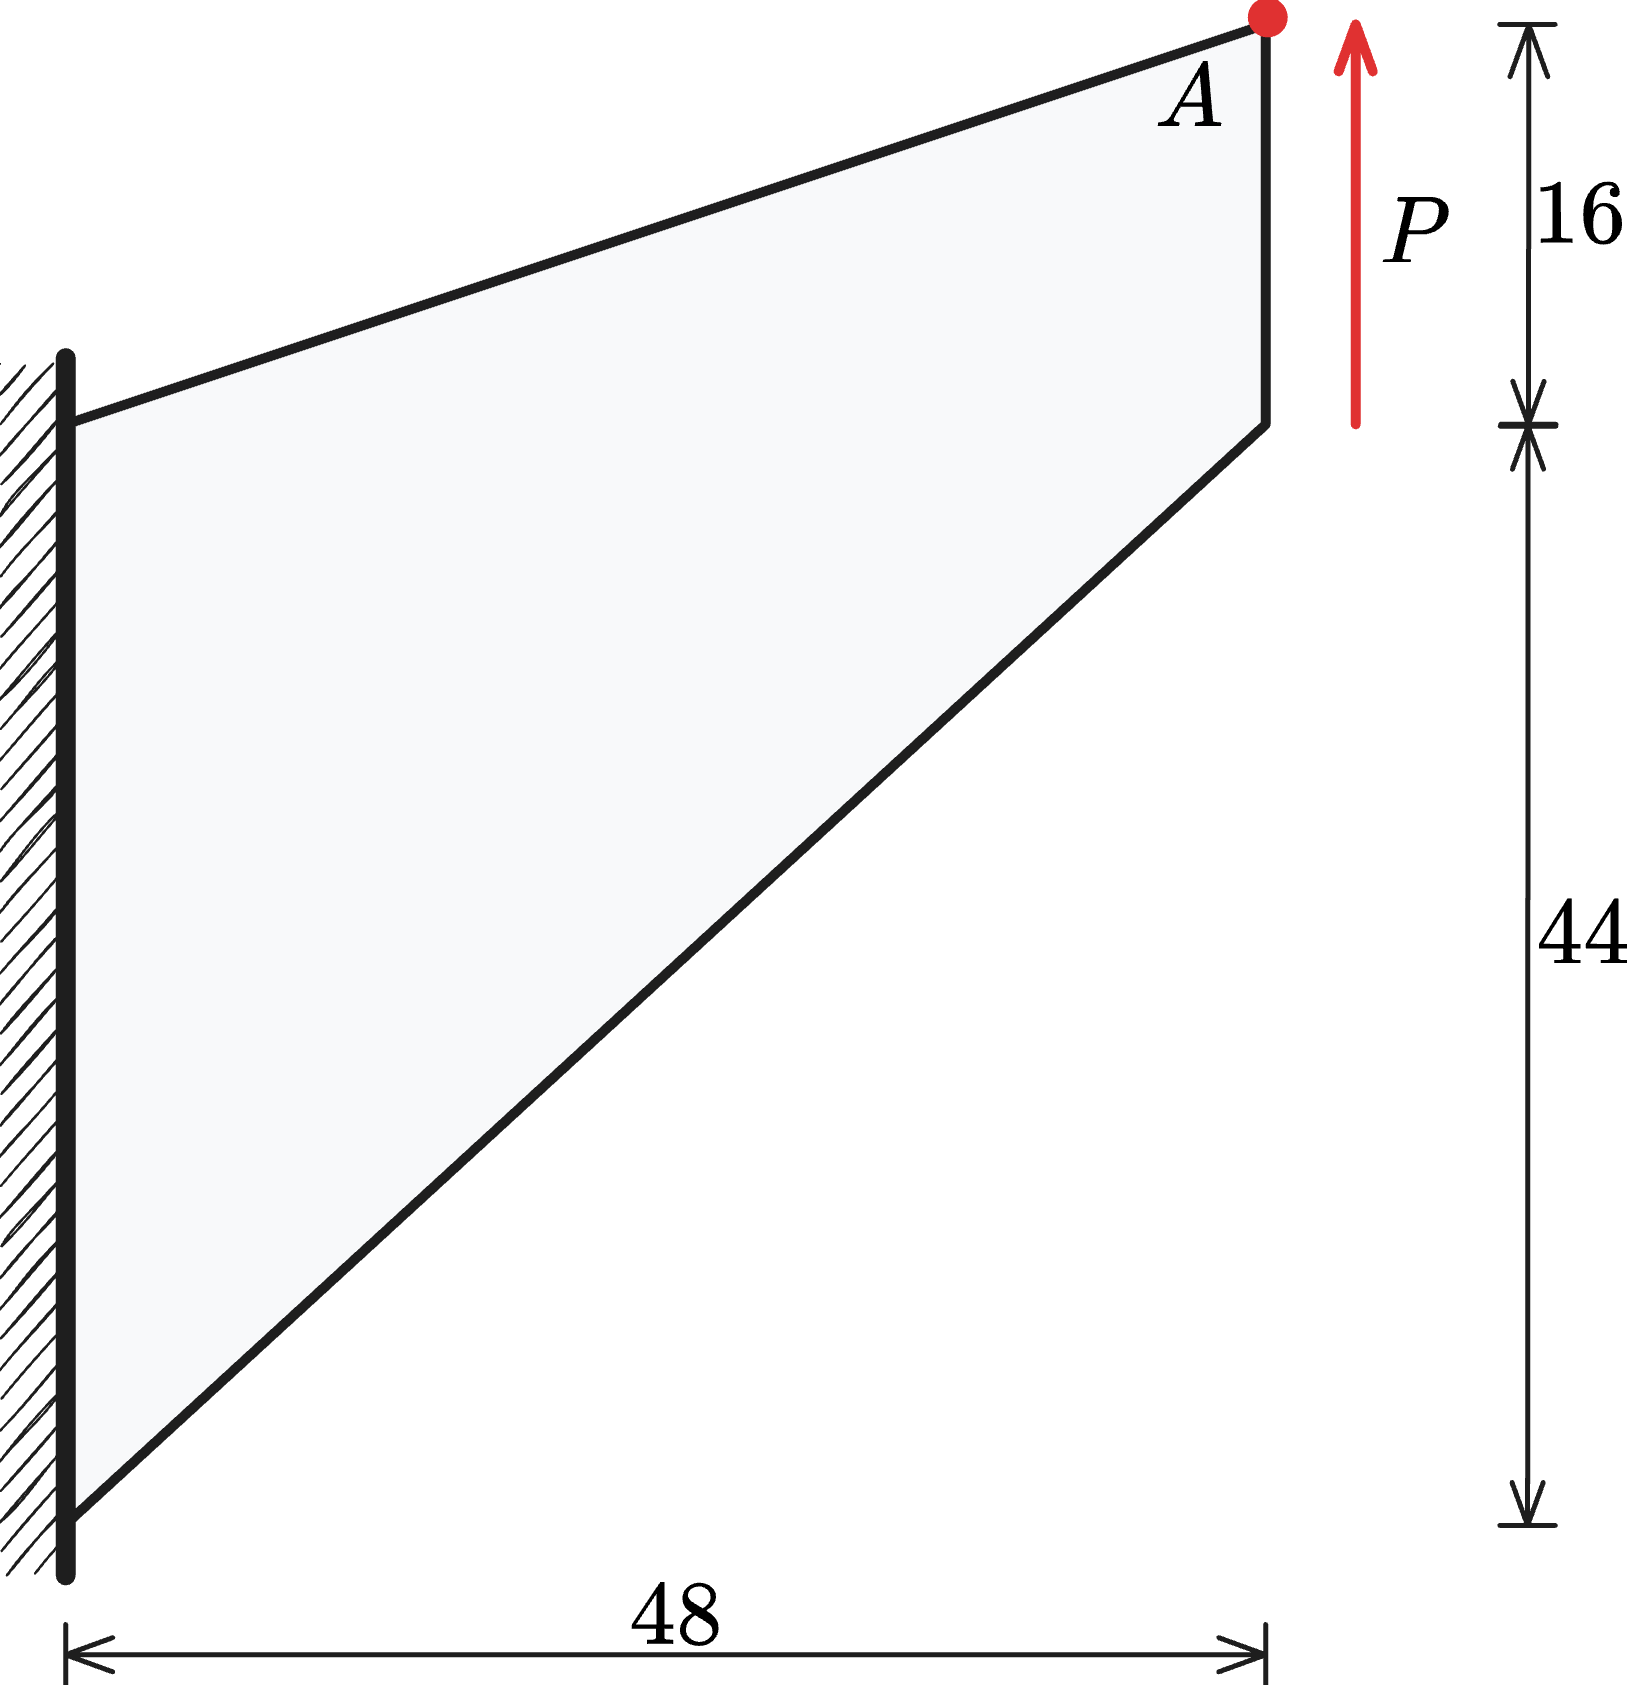
\includegraphics[width=0.6\textwidth]{png/cook_membrane_model.png}
\caption{Illustration of cook membrane problem}\label{cook_illsutration}
\end{figure}


\begin{figure}[!ht]
\centering
% \includegraphics[width=\textwidth]{}
\caption{Illustration of block under compression problem}\label{block_illsutration}
\end{figure}

\begin{figure}[!ht]
\centering
% \includegraphics[width=\textwidth]{}
\caption{Convergence comparison of block under compression problem}\label{block_convergence}
\end{figure}

\begin{figure}[!ht]
\centering
% \includegraphics[width=\textwidth]{}
\caption{Contour plots of block under compression problem}\label{block_contour}
\end{figure}
